% -*- TeX:UTF-8 -*-
%%
%% KAIST 학위논문양식 LaTeX용 (ver 0.5)
%%
%% FINAL English manuscript — assembled from the Notion "_eng" pages.
%% References are left as ~\cite{...}; the .bib will be supplied separately.
%% Figures are NOT inserted yet — each figure location is marked with a
%% placeholder box carrying the intended caption/title.
%%

\documentclass[master,english,final]{kaist-ucs}

% 추가 패키지
\usepackage{amsmath, amssymb}
\usepackage{booktabs}

% @command title 논문 제목
\title[korean] {관상동맥 파열위험지표 정의 및 민감도 분석}
\title[english]{Definition of a Coronary Plaque Rupture Risk Index and Its Sensitivity Analysis}

% @command author 저자 이름
\author[korean]{김}{세 혁}
\author[korean2]{김}{세혁}
\author[chinese]{金}{世 赫}
\author[english]{Kim}{Sehyeog}

% @command advisor 지도교수 이름
\advisor[major]{김 현 진}{Hyun Jin Kim}{signed}
\advisor[major2]{김현진}{Hyun Jin Kim}{signed}
\advisorinfo{Professor of Mechanical Engineering}

% @command department
\department{ME}{engineering}{c}

% @command referee 심사위원
\referee[1]{김 현 진}
\referee[2]{유 승 화}
\referee[3]{이 익 진}

\approvaldate{2026}{05}{27}
\refereedate{2026}{05}{27}
\gradyear{2026}

% Figure placeholder helper — draws a labelled box where a figure will go.
\newcommand{\figplaceholder}[1]{%
  \fbox{\parbox[c][3.2cm][c]{0.9\textwidth}{\centering\textbf{[FIGURE PLACEHOLDER]}\\[4pt]#1}}%
}

% 본문 시작
\begin{document}

\thesisinfo

%% 한글 초록: 500자 미만
\begin{summary}
관상동맥 플라크 파열은 급성 관상동맥 증후군의 주된 원인이며 형태, 혈류역학, 재료 세 인자군이 복합적으로 작용한다.
완전 연성 맥동 유체-고체 연성 해석의 높은 계산 비용으로 인해 세 인자군을 동시에 대규모로 다룬 연구는 부재하였다.
본 학위논문은 첫째, 맥동 하중의 시간 성분과 공간 성분을 분리하여 완전 연성 해석 대비 30배 이상의 비용 절감과 최대 4.5\% 수준의
응력 오차를 달성하는 비용효율적 유체-고체 연성 해석 기법을 제안하고 검증하였다.
둘째, 위 방법을 사용하여 저감쇠 플라크와 석회화 플라크의 대규모 라틴 하이퍼큐브 데이터셋을 구축하고,
응력과 강도의 비로 정의한 여섯 개 취약성 지수를 임상 일곱 기준으로 선별하였으며, 가우시안 과정 회귀 대리모델과 소볼 전역 민감도 분석으로 세 인자군의 기여를 정량화하였다.
결과적으로 맥동 응력 진폭에 강도 정규화를 결합한 두 지수만이 임상적으로 일관되며, 재료물성이 파열 위험의 지배 인자군임을 규명하였다.
\end{summary}

\begin{Korkeyword}
관상동맥 플라크 파열, 유체-고체 연성 해석, 취약성 지수, 전역 민감도 분석, 가우시안 과정 회귀, 섬유막 강성
\end{Korkeyword}

%% 영문 초록: 300단어 미만
\begin{abstract}
Coronary plaque rupture is the leading cause of acute coronary syndrome, arising from the combined action of three factor groups: morphology, hemodynamics, and material properties. Because of the high computational cost of fully coupled pulsatile fluid--structure interaction (FSI) analysis, no prior study has addressed all three factor groups simultaneously at large scale. This thesis makes two contributions. First, it proposes and validates a cost-effective FSI scheme that decouples the temporal and spatial components of pulsatile loading, achieving more than a 30-fold reduction in computational cost relative to fully coupled FSI while keeping the maximum stress error within 4.5\%.
Second, using this scheme, large-scale Latin Hypercube datasets are constructed for low-attenuation and calcified plaques; six vulnerability indices, defined as stress-to-strength ratios, are screened against seven clinical criteria; and the contributions of the three factor groups are quantified using Gaussian process regression surrogate models together with Sobol global sensitivity analysis. The results show that only two indices---those combining pulsatile stress amplitude with strength normalization---are clinically consistent, and material properties are identified as the dominant factor group governing rupture risk.
\end{abstract}

\begin{Engkeyword}
Coronary plaque rupture, Fluid--structure interaction, Vulnerability index, Global sensitivity analysis, Gaussian process regression, Fibrous-cap stiffness
\end{Engkeyword}

\addtocounter{pagemarker}{1}
\newpage

\tableofcontents
\listoftables
\listoffigures


%%======================================================================
%% Chapter 1. Introduction
%%======================================================================
\chapter{Introduction}

\section{Plaque rupture and acute coronary syndrome}
Atherosclerotic plaque is a pathological lesion formed by the accumulation of a lipid-rich necrotic core, fibrous tissue, calcification, and other components within the arterial intima~\cite{bentzon2014, otsuka2016}. As plaque develops, it narrows the vascular lumen and reduces myocardial blood supply, which can ultimately lead to myocardial ischemia~\cite{bentzon2014}. Ischemic heart disease remains the leading single cause of death worldwide and has been reported to account for approximately 9.1 million deaths annually~\cite{WHO2024Top10}.

A fibrous cap separates the necrotic core from the lumen. Plaque rupture refers to the mechanical disruption of this fibrous cap~\cite{virmani2000, otsuka2016}. Once rupture occurs, the highly thrombogenic necrotic core is exposed to the circulating blood, triggering platelet aggregation and rapid thrombus formation, which may result in acute luminal obstruction~\cite{otsuka2016}. Plaque rupture is a major underlying mechanism of acute coronary syndrome (ACS) and can lead to acute myocardial infarction and cardiovascular death~\cite{lee2019, otsuka2016}.

\section{Factors associated with plaque rupture}
From a clinical and pathophysiological perspective, plaque rupture is the result of complex interactions among patient-level clinical risk factors, local biological processes, morphological characteristics, and hemodynamic conditions. Patient-level clinical risk factors such as smoking, dyslipidemia, diabetes, and hypertension contribute to plaque development and destabilization, whereas local biological processes, including inflammation, macrophage infiltration, extracellular matrix degradation, and calcification, modulate fibrous cap stability~\cite{naghavi2003vulnerable, finn2010vulnerable, bentzon2014}. Morphological characteristics, including a thin fibrous cap, a large necrotic core, stenosis severity, and plaque burden, are also strongly associated with plaque vulnerability~\cite{bentzon2014, virmani2006}. In addition, hemodynamic indices such as wall shear stress (WSS), axial plaque stress (APS), and the lesion-specific drop in coronary computed tomography angiography-derived fractional flow reserve ($\Delta \mathrm{FFR}_{CT}$) have been shown to independently predict culprit lesions of ACS beyond conventional morphological features~\cite{lee2019emerald, yang2021}.

To quantitatively assess plaque rupture risk beyond clinical observation alone, computational studies have sought to translate clinical, morphological, and hemodynamic vulnerability features into mechanical quantities. From a mechanical perspective, plaque rupture can be interpreted either as an acute failure event that occurs when the local stress exceeds the tissue strength~\cite{choi2015aps, brown2016, gu2022}, or as a fatigue-driven failure process caused by repeated cyclic blood pressure loading~\cite{bank2000, versluis2006}. Accordingly, previous computational studies have reduced clinically observed vulnerability factors into mechanical determinants: biological changes are represented by material properties and tissue strength, morphological features by stress concentration, and hemodynamic conditions by external loading~\cite{brown2016, gu2022, corti2022}.

\section{Vulnerability index}
Computational studies for quantifying plaque rupture risk have primarily focused on fibrous cap stress, which can be interpreted from two mechanical perspectives: static failure and fatigue failure. From the static failure perspective, rupture is assumed to occur when the maximum stress acting on the fibrous cap during the cardiac cycle exceeds the tissue strength. Accordingly, plaque structural stress (PSS), particularly the peak systolic stress, has been widely used as a representative risk indicator~\cite{teng2014, huang2001}. In contrast, from the fatigue failure perspective, rupture is considered to result from progressive damage accumulation under repeated cyclic loading during each heartbeat~\cite{bank2000, versluis2006}. In this case, the dominant mechanical quantity is not the absolute maximum stress, but the stress amplitude over the cardiac cycle, namely the plaque structural stress variation ($\Delta$PSS)~\cite{costopoulos2017}.

However, plaque vulnerability is governed not only by the magnitude of mechanical stress but also by the load-bearing capacity of the fibrous cap. Thus, for a given stress level, a lower fibrous cap strength increases the likelihood that local stress will exceed tissue strength~\cite{corti2022, brown2016, gu2022}. The fibrous cap strength is known to vary considerably among patients because it depends on biological and microstructural characteristics, including collagen content and tissue organization~\cite{savvopoulos2024afm, chai2013}.

\section{Limitations of previous studies}
To improve the predictive capability of plaque rupture risk indicators, it is necessary not only to identify individual factors associated with rupture, but also to quantitatively determine which group of factors primarily governs the variability of the vulnerability index. This is directly related to the clinical question of which factors should be prioritized for measurement and incorporated into risk stratification~\cite{virmani2006, lee2019emerald, saltelli2008}.

However, previous computational studies have generally been limited to partial combinations of the relevant factor groups rather than simultaneously varying all three categories. Many studies have focused only on morphological factors~\cite{cilla2012}, while others have considered combinations of morphology and composition~\cite{costopoulos2017, teng2014, milzi2021} or morphology and material properties~\cite{polzer2019, stefanati2024}. Although some studies have performed fluid--structure interaction (FSI) analyses that incorporate both blood flow and arterial wall deformation to account for all three factor groups, the number of simulated cases has typically been limited to only several or a few dozen~\cite{zhao2024}. Such sample sizes are insufficient to achieve the statistical convergence required for reliable global sensitivity analysis (GSA).

The fundamental reason for this limitation is the substantial computational cost of pulsatile FSI analysis. Simultaneously accounting for material properties, plaque morphology, and hemodynamic loading requires coupled fluid--structure simulations under time-varying physiological pressure and flow conditions, which are computationally expensive~\cite{wang2021_multipatient, lissoni2025_coronary_methods}. As a result, previous studies have not yet systematically identified the dominant determinants of plaque rupture risk by simultaneously analyzing all three factor groups under pulsatile loading with a sufficiently large sample size.

\section{Present study}
This study addresses the above limitation by combining two complementary components: the development of a cost-efficient computational method for pulsatile plaque stress analysis and a large-scale sensitivity analysis of plaque rupture risk.

First, we develop and validate a computationally efficient strategy for pulsatile FSI-based stress analysis. To reduce the computational burden associated with fully coupled pulsatile FSI simulations, we propose an alternative approach that separates the temporal and spatial components of pulsatile loading. This enables pulsatile stress analysis to be performed for a large number of plaque models at a feasible computational cost.

Second, using the proposed computationally efficient FSI, we perform a large-scale global sensitivity analysis under pulsatile loading. Plaque rupture risk is quantified using vulnerability indices defined as the ratio of mechanical stress to fibrous cap strength, $\mathrm{VI} = \mathrm{stress}/\mathrm{strength}$. Both static and fatigue failure mechanisms are considered by using PSS and $\Delta\mathrm{PSS}$ as stress measures, respectively. Material properties, morphological characteristics, and hemodynamic loading parameters are then varied simultaneously to determine their relative contributions to the variability of the vulnerability indices.

By integrating these two components, this study presents a unified in-silico framework for evaluating plaque rupture risk and quantitatively identifying the dominant mechanical determinants of plaque vulnerability.


%%======================================================================
%% Chapter 2. Computationally Efficient FSI
%%======================================================================
\chapter{Computationally Efficient Fluid--Structure Interaction (FSI)}

\section{Framework}
The central idea of the proposed method is to decouple the temporal and spatial components of pulsatile loading. Specifically, for given pulsatile fluid and structural boundary conditions, the local vascular wall stress field at a target time point $t_a$ within the cardiac cycle, $\sigma(t_a)$, is approximated by combining a single pulsatile one-dimensional (1D) reduced-order model (ROM) analysis with steady three-dimensional fluid and structural analyses evaluated at that target time point. This approach is based on the observation that biomechanical indices at representative time points, such as peak systole or end diastole, can provide diagnostically relevant information. Therefore, the proposed method estimates the instantaneous stress state at selected target time points without solving the full time-dependent coupled problem.

In this framework, the ROM represents the vascular system as an axial 1D network and computes time-varying pressure and flow waveforms throughout the vascular tree at low computational cost. However, a purely 1D representation may not fully capture pressure losses in geometrically complex regions, such as stenoses and bifurcations. Therefore, physics-based correction terms are incorporated to represent the pressure drop in these regions as a nonlinear function of flow rate~\cite{choi2025rom}.

\begin{figure}[!htbp]
\centering
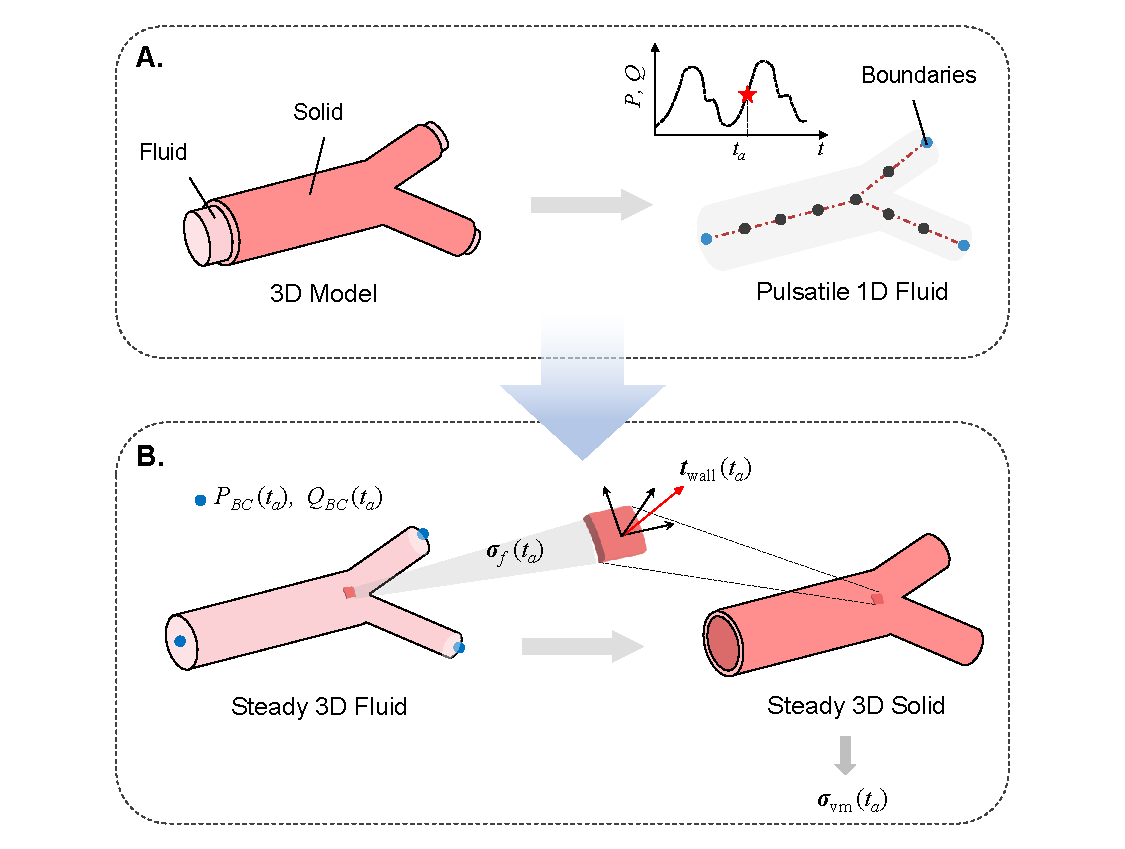
\includegraphics[width=\textwidth,height=0.82\textheight,keepaspectratio]{figures/figure_page_01.pdf}
\caption[Cost-effective FSI framework]{Schematic framework of the proposed computationally efficient FSI method combining 1D pulsatile ROM analysis (A) with 3D steady fluid and quasi-static structural analysis (B).}
\label{fig:cefsi-framework}
\end{figure}

As shown in Figure~\ref{fig:cefsi-framework}, the procedure consists of a pulsatile analysis followed by steady analyses and is divided into three steps.

\textbf{Step 1 (pulsatile analysis, A).} A pulsatile 1D ROM simulation is performed for the given geometry and boundary conditions to compute time-varying pressure and flow waveforms at the vascular boundaries. The boundary values are then extracted at the target time point $t_a$.

\textbf{Step 2 (steady fluid analysis, B).} A three-dimensional steady fluid analysis is performed using the boundary conditions at $t_a$ to compute the wall traction required for the subsequent stress analysis.

\textbf{Step 3 (quasi-static structural analysis, B).} A three-dimensional quasi-static structural analysis is performed by applying the computed wall traction, yielding the stress and displacement fields at $t_a$.

Thus, the computationally expensive pulsatile analysis is performed only once in the 1D domain, whereas the stress fields at selected target time points are obtained by repeating Steps 2 and 3 as three-dimensional steady or quasi-static snapshot analyses.

\section{Governing equations}
This section describes the governing equations for each of the three steps and then presents the governing equations of the reference fully coupled FSI model used for validation.

\subsection{One-dimensional reduced-order hemodynamics (Step 1)}
In Step 1, the vascular system is reduced to an axial 1D network to compute pulsatile blood flow. The conserved variables of the 1D model are the cross-sectional area $S(z,t)$, cross-sectionally averaged flow rate $Q(z,t)$, and cross-sectionally averaged pressure $P(z,t)$. The mass and momentum conservation equations are written as Eqs.~(1) and (2):

\begin{equation}
\frac{\partial S}{\partial t} + \frac{\partial Q}{\partial z} = 0
\end{equation}

\begin{equation}
\frac{\partial Q}{\partial t} + \frac{\partial}{\partial z}\!\left(\frac{\alpha Q^2}{S}\right) + \frac{S}{\rho}\frac{\partial P}{\partial z} = -\frac{NQ}{S}
\end{equation}

where $z$ is the axial coordinate, $\rho$ is the blood density, $\alpha$ is the momentum correction coefficient, and $N$ is the viscous resistance term. In this study, a rigid-wall assumption is used in the 1D analysis; therefore, the cross-sectional area $S$ does not vary with time, and Eq.~(1) reduces to $\partial Q/\partial z = 0$. Assuming a parabolic velocity profile, $\alpha = 4/3$ and $N = 8\pi\nu$, where $\nu$ is the kinematic viscosity of blood.

Although Eqs.~(1) and (2) efficiently capture global pulsatile hemodynamics, additional pressure losses arise in regions with large local geometric variations, such as stenoses and bifurcations. To account for these effects, a physics-based ROM correction term that expresses the pressure drop as a nonlinear function of flow rate is incorporated, as shown in Eq.~(3)~\cite{choi2025rom}:

\begin{equation}
\Delta P = aQ + bQ^2 + c\frac{dQ}{dt}
\end{equation}

The coefficients $a$, $b$, and $c$ represent viscous loss, nonlinear convective loss, and unsteady inertial effects, respectively, and are identified through a preprocessing procedure for each geometry~\cite{choi2025rom}.

\subsection{Three-dimensional steady fluid problem (Step 2)}
In Step 2, a three-dimensional steady fluid analysis is performed using the pressure or flow boundary conditions extracted from the ROM at the target time point $t_a$. Blood is assumed to be an incompressible Newtonian fluid~\cite{ku1997blood}. In the fluid domain $\Omega_f$, the mass and momentum conservation equations are given by Eqs.~(4) and (5):

\begin{equation}
\nabla \cdot \mathbf{u}_f = 0 \quad \text{in } \Omega_f
\end{equation}

\begin{equation}
\rho_f \left[\frac{\partial \mathbf{u}_f}{\partial t} + (\mathbf{u}_f \cdot \nabla)\mathbf{u}_f\right] = \nabla \cdot \boldsymbol{\sigma}_f \quad \text{in } \Omega_f
\end{equation}

where $\mathbf{u}_f$ is the fluid velocity, $\rho_f$ is the blood density, and $\boldsymbol{\sigma}_f$ is the fluid Cauchy stress tensor. Because Step 2 approximates the instantaneous state at $t_a$ as a steady state, the transient term $\partial \mathbf{u}_f/\partial t$ is omitted from Eq.~(5). The stress tensor of an incompressible Newtonian fluid is defined as Eq.~(6):

\begin{equation}
\boldsymbol{\sigma}_f = -p\mathbf{I} + \mu_f\left(\nabla\mathbf{u}_f + \nabla\mathbf{u}_f^{T}\right)
\end{equation}

where $p$ is the pressure, $\mu_f$ is the dynamic viscosity of blood, and $\mathbf{I}$ is the identity tensor. The three-dimensional fluid analysis provides the fluid traction on the vascular wall surface $\Gamma_{wall}$, as given by Eq.~(7):

\begin{equation}
\mathbf{t}_{wall}^{f}(t_a) = \boldsymbol{\sigma}_f(t_a)\,\mathbf{n}_f \quad \text{on } \Gamma_{wall}
\end{equation}

where $\mathbf{n}_f$ is the outward unit normal vector defined on the fluid domain.

\subsection{Three-dimensional quasi-static structural problem (Step 3)}
In Step 3, the wall traction computed in Step 2 is mapped to the inner wall surface of the solid domain, and a quasi-static structural analysis is performed. In the solid domain $\Omega_s$, the quasi-static equilibrium equation is given by Eq.~(8):

\begin{equation}
\nabla \cdot \boldsymbol{\sigma}_s + \mathbf{f}_s = 0 \quad \text{in } \Omega_s
\end{equation}

where $\boldsymbol{\sigma}_s$ is the solid Cauchy stress tensor and $\mathbf{f}_s$ is the body force. In this study, body forces are neglected, such that $\mathbf{f}_s = 0$. Because coronary wall deformation is assumed to remain small in this study, the vascular wall is modeled as an isotropic linear elastic material~\cite{cheng1993}. Under the small-deformation assumption, higher-order terms in the displacement gradient are neglected, and the strain is approximated by the infinitesimal strain tensor~\cite{boresi2003}. Accordingly, the strain--displacement relation, linear elastic constitutive equation, and Lam\'e constants are given by Eqs.~(9)--(12):

\begin{equation}
\boldsymbol{\varepsilon}_s = \frac{1}{2}\left(\nabla\mathbf{d}_s + \nabla\mathbf{d}_s^{T}\right)
\end{equation}

\begin{equation}
\boldsymbol{\sigma}_s = \lambda_s\,\mathrm{tr}(\boldsymbol{\varepsilon}_s)\mathbf{I} + 2\mu_s\boldsymbol{\varepsilon}_s
\end{equation}

\begin{equation}
\lambda_s = \frac{E_s\nu_s}{(1 + \nu_s)(1 - 2\nu_s)}
\end{equation}

\begin{equation}
\mu_s = \frac{E_s}{2(1 + \nu_s)}
\end{equation}

Here, $\mathbf{d}_s$ is the solid displacement field, $\boldsymbol{\varepsilon}_s$ is the infinitesimal strain tensor, $\lambda_s$ and $\mu_s$ are the Lam\'e constants, and $E_s$ and $\nu_s$ are Young's modulus and Poisson's ratio, respectively. The traction boundary condition imposed on the structural domain at the fluid--structure interface is given by Eq.~(13):

\begin{equation}
\boldsymbol{\sigma}_s \mathbf{n}_s = -\mathbf{t}_{wall}^{f}(t_a) \quad \text{on } \Gamma_{wall}
\end{equation}

where $\mathbf{n}_s$ is the outward unit normal vector of the solid domain. Displacement constraints are applied at the inlet and outlet cross-sections to remove rigid-body motion.

\subsection{Reference fully coupled FSI formulation}
In the reference fully coupled FSI model, the fluid domain is described using an arbitrary Lagrangian--Eulerian (ALE) formulation, and the Navier--Stokes equations are solved on the moving fluid mesh, as given by Eqs.~(14) and (15):

\begin{equation}
\nabla \cdot \mathbf{u}_f = 0 \quad \text{in } \Omega_f(t)
\end{equation}

\begin{equation}
\rho_f \left[\frac{\partial \mathbf{u}_f}{\partial t} + \left((\mathbf{u}_f - \mathbf{w}) \cdot \nabla\right)\mathbf{u}_f\right] = \nabla \cdot \boldsymbol{\sigma}_f \quad \text{in } \Omega_f(t)
\end{equation}

where $\mathbf{w}$ is the ALE mesh velocity. In the solid domain, the structural dynamics equation is solved using the same isotropic linear elastic constitutive model described in Section~2.2.3, as given by Eq.~(16):

\begin{equation}
\rho_s \frac{\partial^2 \mathbf{d}_s}{\partial t^2} = \nabla \cdot \boldsymbol{\sigma}_s + \mathbf{f}_s \quad \text{in } \Omega_s(t)
\end{equation}

At the fluid--structure interface $\Gamma_{fs}$, the continuity of velocity and traction is imposed as Eqs.~(17) and (18):

\begin{equation}
\mathbf{u}_f = \frac{\partial \mathbf{d}_s}{\partial t} \quad \text{on } \Gamma_{fs}
\end{equation}

\begin{equation}
\boldsymbol{\sigma}_f \mathbf{n}_f + \boldsymbol{\sigma}_s \mathbf{n}_s = 0 \quad \text{on } \Gamma_{fs}
\end{equation}

\section{Validation setup}
\subsection{Geometries}
The proposed method was validated using three geometries with increasing anatomical and hemodynamic complexity (Figure~\ref{fig:geo_ROMFSI}). First, the idealized left anterior descending (LAD) coronary artery was modeled as a simple cylindrical segment with a total length of $L=10$~cm, a lumen radius of $R=0.1$~cm, and a wall thickness of $t=0.02$~cm. To mimic stenotic disease, an eccentric stenosis with a degree of stenosis (DOS) of 55\% was introduced in the distal segment. Second, a patient-specific abdominal aortic aneurysm (AAA) geometry was reconstructed from CT images. The AAA model had a maximum luminal diameter of approximately 10~cm and two outlets (b and c). Third, a patient-specific coronary artery geometry was reconstructed from CT images. This model included serial triple stenoses extending from the left main coronary artery (LM) to the mid- and distal LAD, with stenosis severities of 68\%, 69\%, and 70\%, respectively (mean, 69\%). The fluid and solid domains were discretized using unstructured tetrahedral meshes generated with the TetGen-based meshing module in SimVascular~\cite{updegrove2017simvascular, si2015tetgen}. Three boundary-layer mesh layers were added near the wall in the fluid domain to resolve near-wall flow.

\begin{figure}[!htbp]
\centering
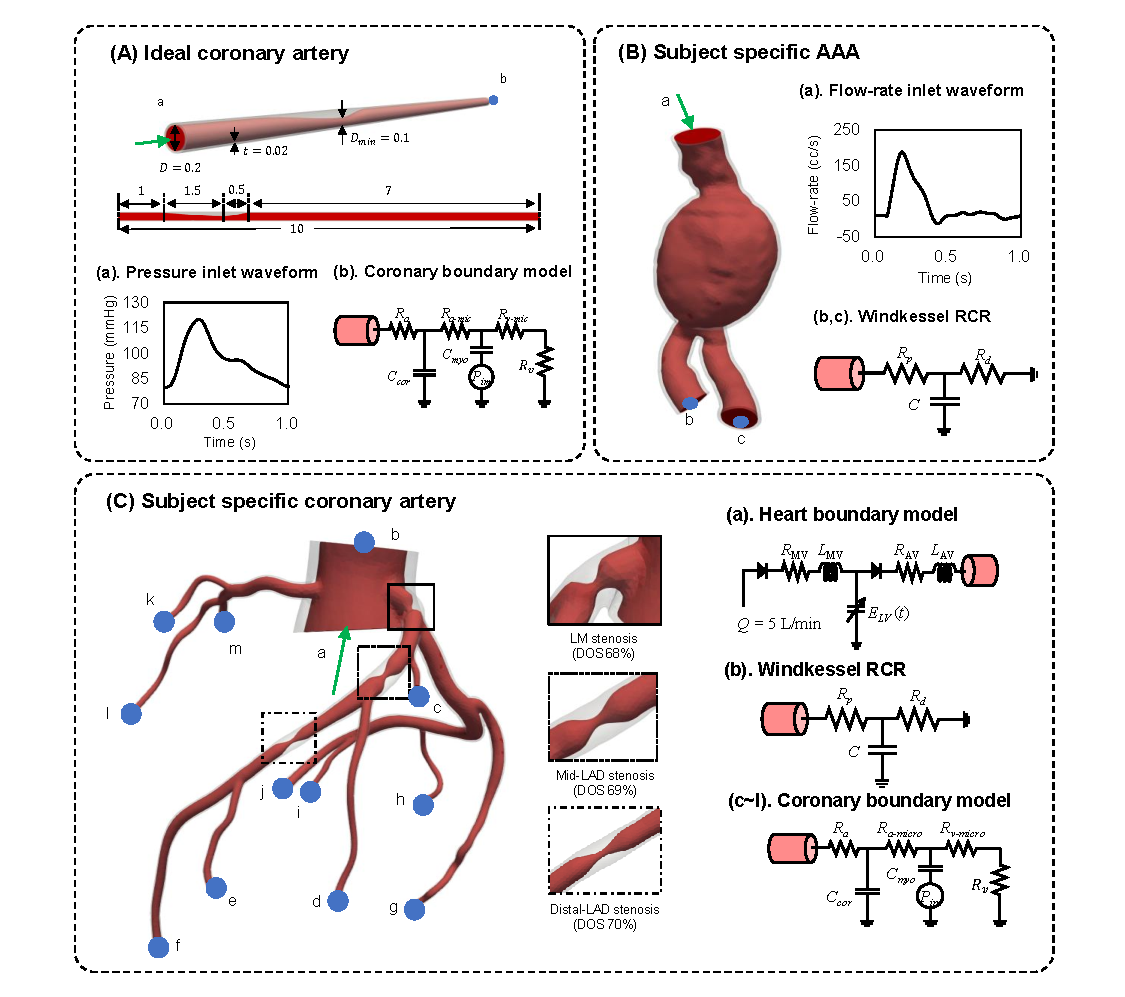
\includegraphics[width=\textwidth,height=0.82\textheight,keepaspectratio]{figures/figure_page_02.pdf}
\caption[Idealized coronary and subject-specific geometries]{Geometries and boundary conditions used for validation of the proposed computationally efficient FSI method: (A) idealized coronary artery, (B) patient-specific abdominal aortic aneurysm (AAA), and (C) patient-specific coronary artery.}
\label{fig:geo_ROMFSI}
\end{figure}

\subsection{Material properties}
The solid and fluid material properties used in the validation models were assigned based on literature values and were treated as fixed values under the linear elastic assumption. The solid material properties are summarized in Table~\ref{tab:validation-material}.

\begin{table}[ht]
\caption[Validation material properties]{Validation material properties.}
\label{tab:validation-material}
\begin{center}
\begin{tabular}{lllll}
\hline\hline
Target & $E$ & $\nu$ & $\rho$ & Reference \\
\hline
Coronary wall & $1.0\times10^{7}$ dyn/cm$^2$ & 0.45 & 1.1 g/cm$^3$ & \cite{cheng1993, hsu2014, chen2021ldl, jiang2022} \\
AAA wall & $6.0\times10^{7}$ dyn/cm$^2$ & 0.49 & 1.0 g/cm$^3$ & \cite{joldes2016, figueroa2006} \\
\hline\hline
\end{tabular}
\end{center}
\end{table}

Blood in the fluid domain was modeled as an incompressible Newtonian fluid with a density of 1.06~g/cm$^3$ and a dynamic viscosity of $\mu=0.04$~poise~\cite{ku1997blood}.

\subsection{Boundary conditions}
Fluid boundary conditions for each geometry were prescribed based on previous studies, as shown in Figure~\ref{fig:geo_ROMFSI}. For the idealized LAD coronary artery (A), a pulsatile inlet pressure waveform representative of an average adult male (120/80~mmHg) and a lumped-parameter coronary outlet boundary condition were prescribed~\cite{guyton2011_av_P, kim2010coronary}. For the patient-specific AAA model (B), a time-varying flow waveform measured by MRI was prescribed at the inlet, and Windkessel RCR models were applied at the outlets~\cite{westerhof2009windkessel}. For the patient-specific coronary artery model (C), the inlet was coupled to a lumped-parameter heart boundary model that represents left ventricular pressure generation and the opening and closure of the mitral and aortic valves~\cite{kim2010coronary}. Coronary outlet boundary conditions were prescribed at the coronary branches, whereas a Windkessel RCR model was applied only at the aortic outlet (b). The parameter values for models A and B are summarized in Table~\ref{tab:bc-ideal-aaa}, and those for model C are summarized in Tables~\ref{tab:bc-heart-aorta} and~\ref{tab:bc-subject-coronary}.

\begin{table}[ht]
\caption[Ideal coronary and AAA boundary conditions]{Ideal coronary \& AAA boundary-condition coefficients.}
\label{tab:bc-ideal-aaa}
\begin{center}
\begin{tabular}{lllr}
\hline\hline
Model & Parameter & Value & Unit \\
\hline
Ideal coronary & $R_a$ & 78827 & dyn$\cdot$s/cm$^5$ \\
(outlet b) & $C_a$ & $0.396\times10^{-6}$ & cm$^5$/dyn \\
& $R_{a\text{-micro}}$ & 128094 & dyn$\cdot$s/cm$^5$ \\
& $C_{im}$ & $3.20\times10^{-5}$ & cm$^5$/dyn \\
& $R_v$ & 19706 & dyn$\cdot$s/cm$^5$ \\
& $R_{v\text{-micro}}$ & 19706 & dyn$\cdot$s/cm$^5$ \\
& inlet & prescribed pressure (70--130 mmHg) & --- \\
AAA & $R_p$ & 450.0 & dyn$\cdot$s/cm$^5$ \\
(outlets b, c) & $C$ & $5.0\times10^{-4}$ & cm$^5$/dyn \\
& $R_d$ & 6820.0 & dyn$\cdot$s/cm$^5$ \\
& inlet & prescribed flow-rate waveform & --- \\
\hline\hline
\end{tabular}
\end{center}
\end{table}

\begin{table}[ht]
\caption[Subject-specific coronary inlet and aortic outlet BC]{Subject-specific coronary: heart inlet model (a) and aortic Windkessel RCR (b) coefficients.}
\label{tab:bc-heart-aorta}
\begin{center}
\begin{tabular}{lllr}
\hline\hline
Model & Parameter & Value & Unit \\
\hline
Heart inlet (a) & $CO$        & 5.0    & L/min \\
                & $t_{cycle}$ & 1.0    & s \\
                & $t_{sys}$   & 0.33   & s \\
                & $R_{LA}$    & 5.0    & --- \\
                & $L_{LA}$    & 1.0    & --- \\
                & $R_{LV}$    & 10.0   & --- \\
                & $L_{LV}$    & 10.0   & --- \\
                & $E_{max}$   & 2.0    & mmHg/cc \\
Aortic Windkessel RCR (b) & $R_p$ & 232.44              & dyn$\cdot$s/cm$^5$ \\
                          & $C$   & $1.50\times10^{-3}$ & cm$^5$/dyn \\
                          & $R_d$ & 1317.18             & dyn$\cdot$s/cm$^5$ \\
\hline\hline
\end{tabular}
\end{center}
\end{table}

\begin{table}[ht]
\caption[Subject-specific coronary boundary conditions]{Subject-specific coronary outlets (c--m). Units: $R$ in dyn$\cdot$s/cm$^5$; $C$ in cm$^5$/dyn.}
\label{tab:bc-subject-coronary}
\begin{center}
\small
\begin{tabular}{lrrrll}
\hline\hline
Outlet & $R_a$ & $R_{a\text{-micro}}$ & $R_{v\text{-micro}}$ & $C_a$ & $C_{im}$ \\
\hline
c & 76680 & 128624 & 39576 & $2.86\times10^{-7}$ & $2.31\times10^{-6}$ \\
d & 67588 & 113374 & 34884 & $3.97\times10^{-7}$ & $3.21\times10^{-6}$ \\
e & 65168 & 109315 & 33635 & $4.37\times10^{-7}$ & $3.53\times10^{-6}$ \\
f & 56556 & 94868  & 29190 & $6.31\times10^{-7}$ & $5.11\times10^{-6}$ \\
g & 64918 & 108895 & 33506 & $4.41\times10^{-7}$ & $3.57\times10^{-6}$ \\
h & 70224 & 117796 & 36244 & $3.60\times10^{-7}$ & $2.91\times10^{-6}$ \\
i & 71302 & 119603 & 36801 & $3.45\times10^{-7}$ & $2.79\times10^{-6}$ \\
j & 46302 & 77668  & 23898 & $1.06\times10^{-6}$ & $8.60\times10^{-6}$ \\
k & 66831 & 112104 & 34493 & $7.50\times10^{-7}$ & $6.07\times10^{-6}$ \\
l & 65058 & 109130 & 33578 & $8.04\times10^{-7}$ & $6.51\times10^{-6}$ \\
m & 55847 & 93680  & 28824 & $1.20\times10^{-7}$ & $9.70\times10^{-7}$ \\
\hline\hline
\end{tabular}
\end{center}
\end{table}

\subsection{Computational details}
All three-dimensional simulations, including steady fluid analysis, prestressing, pulsatile rigid-wall fluid analysis, and fully coupled FSI, were performed using svFSI~\cite{zhu2022svfsi}. The 1D ROM simulations were performed using an in-house C++ solver. The three-dimensional simulations were conducted on an HPC cluster equipped with Intel Xeon processors (2 sockets, 96 cores) and 257~GB of RAM, whereas the 1D ROM simulations were performed on a desktop workstation with an Intel Core i7-12700K processor (3.61~GHz) and 64~GB of RAM. To obtain vascular wall prestress, cycle-averaged inlet pressures and outlet flow rates were computed from the converged pulsatile solution and applied to a steady fluid analysis. The resulting time-averaged wall traction was then applied to the structural domain in a prestressing analysis. The obtained prestress field was applied identically in both the fully coupled FSI simulation and the solid analysis of the proposed method~\cite{hsu2011prestress}.

\section{Validation results}
\subsection{Validation metric}
Five representative time points within the cardiac cycle were defined for stress field comparison: $t_1$, end diastole; $t_2$, maximum wall-motion-induced volumetric change rate; $t_3$, peak systole; $t_4$, minimum volumetric change rate; and $t_5$, mid diastole. For the idealized LAD model, an additional time point, $t^{*}$, was included because the acceleration phase did not coincide with the extrema of the volumetric change rate. The accuracy of the proposed method was quantified by comparing the nodal von Mises stress on the same solid mesh, using the fully coupled transient 3D FSI solution based on the ALE formulation as the reference solution. At each target time point $t_a$, the global relative $L_2$-norm error was defined as follows:

\begin{equation}
e_{L2}(t_a) = \frac{\left[\sum_{i=1}^{N}\left(\sigma^{\mathrm{Prop}}_{vm,i}(t_a) - \sigma^{\mathrm{FSI}}_{vm,i}(t_a)\right)^2\right]^{1/2}}{\left[\sum_{i=1}^{N}\left(\sigma^{\mathrm{FSI}}_{vm,i}(t_a)\right)^2\right]^{1/2}}
\end{equation}

where $N$ is the total number of solid nodes.

\subsection{Results}
For all three geometries, the proposed method reproduced the von Mises stress fields of the reference FSI simulation with low global relative $L_2$ errors (Table~\ref{tab:val-l2-error}). Specifically, the errors remained below 1\% for the idealized coronary artery, below 4.5\% for the patient-specific coronary artery, and below 2\% for the AAA model. Across the selected time points, the errors were smallest at end diastole and mid diastole and tended to increase during phases with rapid wall motion. This trend is expected because the rigid-wall approximation deviates most strongly from the compliant FSI response during these phases.

In terms of computational cost, the proposed method achieved an average reduction of more than 220-fold compared with fully coupled 3D FSI (Table~\ref{tab:val-cost}). This reduction was achieved by replacing the fully pulsatile 3D analysis with a combination of 1D reduced-order hemodynamic analysis and steady three-dimensional snapshot analyses. The ramped-flow step was used only once per geometry as a preprocessing step for ROM coefficient identification and was not repeated for additional snapshot evaluations.

\begin{table}[ht]
\caption[L2 error of von Mises stress]{Selected time instants and global relative $L_2$-norm error of von Mises stress.}
\label{tab:val-l2-error}
\begin{center}
\begin{tabular}{lcccccc}
\hline\hline
& \multicolumn{2}{c}{Idealized coronary} & \multicolumn{2}{c}{Subject-specific coronary} & \multicolumn{2}{c}{Subject-specific AAA} \\
Time point & Time (s) & Error (\%) & Time (s) & Error (\%) & Time (s) & Error (\%) \\
\hline
$t_1$: End-diastole & 0.05 & 0.13 & 0.05 & 1.98 & 0.08 & 0.22 \\
$t_2$: Max vol.-change & 0.15 & 0.96 & 0.15 & 3.04 & 0.15 & 1.12 \\
$t_3$: Peak systole & 0.28 & 0.28 & 0.25 & 3.91 & 0.25 & 1.00 \\
$t_4$: Min vol.-change & 0.35 & 0.91 & 0.35 & 4.45 & 0.35 & 0.87 \\
$t_5$: Mid-diastole & 0.80 & 0.15 & 0.70 & 1.62 & 0.70 & 0.30 \\
$t^{*}$: Additional & 0.45 & 0.17 & --- & --- & --- & --- \\
\hline\hline
\end{tabular}
\end{center}
\end{table}

\begin{table}[ht]
\caption[Computational time]{Computational time (min).}
\label{tab:val-cost}
\begin{center}
\begin{tabular}{lrrr}
\hline\hline
Simulation stage & Idealized coronary & Subject-specific coronary & Subject-specific AAA \\
\hline
Ramped-flow$^{a}$ & 3.3 & 33 & 5 \\
1D pulsatile & 0.2 & 3 & 0.9 \\
3D steady fluid & 1.2 & 15 & 7 \\
3D steady solid & 8 & 65 & 21 \\
\textbf{Total (proposed)} & \textbf{12} & \textbf{116} & \textbf{34} \\
Full 3D FSI & 6866 & 9989 & 1030 \\
\hline\hline
\end{tabular}\\
$^{a}$ One-time preprocessing step per geometry.
\end{center}
\end{table}

\begin{figure}[!htbp]
\centering
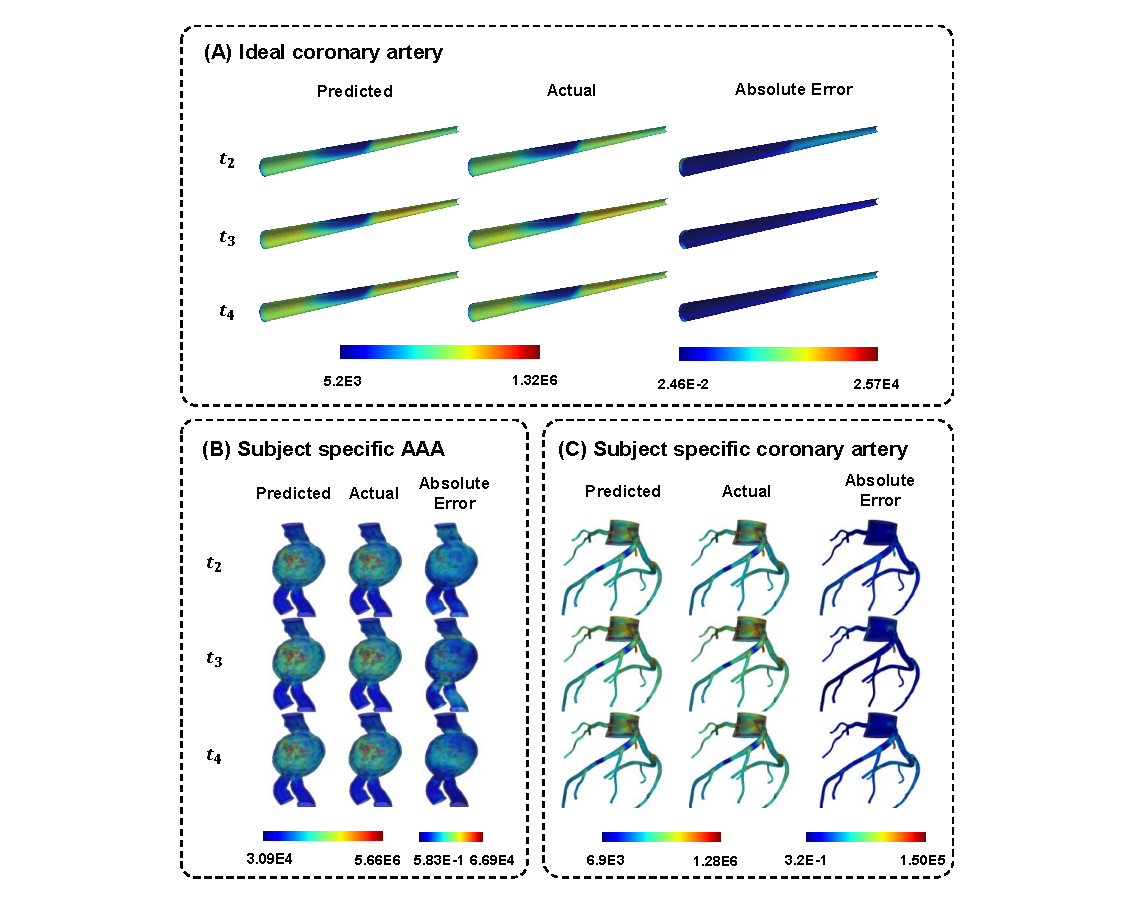
\includegraphics[width=\textwidth,height=0.82\textheight,keepaspectratio]{figures/figure_page_03.pdf}
\caption[Validation results]{Comparison of von Mises stress contours predicted by the proposed computationally efficient FSI method and the reference fully coupled FSI solution for three validation geometries at $t_2$, $t_3$, and $t_4$.}
\label{fig:ch2-validation}
\end{figure}

Figure~\ref{fig:ch2-validation} compares the von Mises stress contours predicted by the proposed computationally efficient FSI method with those obtained from the reference fully coupled FSI simulation at representative time points. For all three validation geometries, the predicted stress fields showed close agreement with the reference FSI results, reproducing both the overall spatial distribution and the regions of elevated stress. The absolute error contours indicate that the discrepancies were generally small relative to the stress magnitude, although localized errors appeared near geometrically complex regions, such as stenoses and bifurcations, and at time points associated with rapid wall motion. These errors are consistent with the steady rigid-wall approximation used in the proposed method, but they did not substantially alter the dominant stress patterns. Therefore, the proposed method provides sufficient accuracy for estimating instantaneous wall stress fields while substantially reducing the computational cost, supporting its use as the forward solver for the large-scale sensitivity analysis in Chapter~3.


%%======================================================================
%% Chapter 3. Parametric Analysis Framework
%%======================================================================
\chapter{Parametric Analysis Framework for Plaque Rupture Risk}

This chapter presents a three-stage parametric analysis framework consisting of data generation, vulnerability-index formulation, and statistical analysis to investigate coronary plaque rupture risk from morphological, hemodynamic, and material perspectives. First, the cost-effective pulsatile FSI model validated in Chapter~2 was used as a forward solver to generate 1{,}000 input--output datasets each for low-attenuation plaques (LAPs) and calcified plaques (CPs). Candidate vulnerability indices (VIs), defined as the ratio of stress to strength, were then formulated and screened according to clinically relevant criteria. Finally, for the selected VI, a Gaussian process regression (GPR)-based surrogate model was trained, and the contribution of each factor group was quantified using Sobol variance-based global sensitivity analysis.

\begin{figure}[!htbp]
\centering
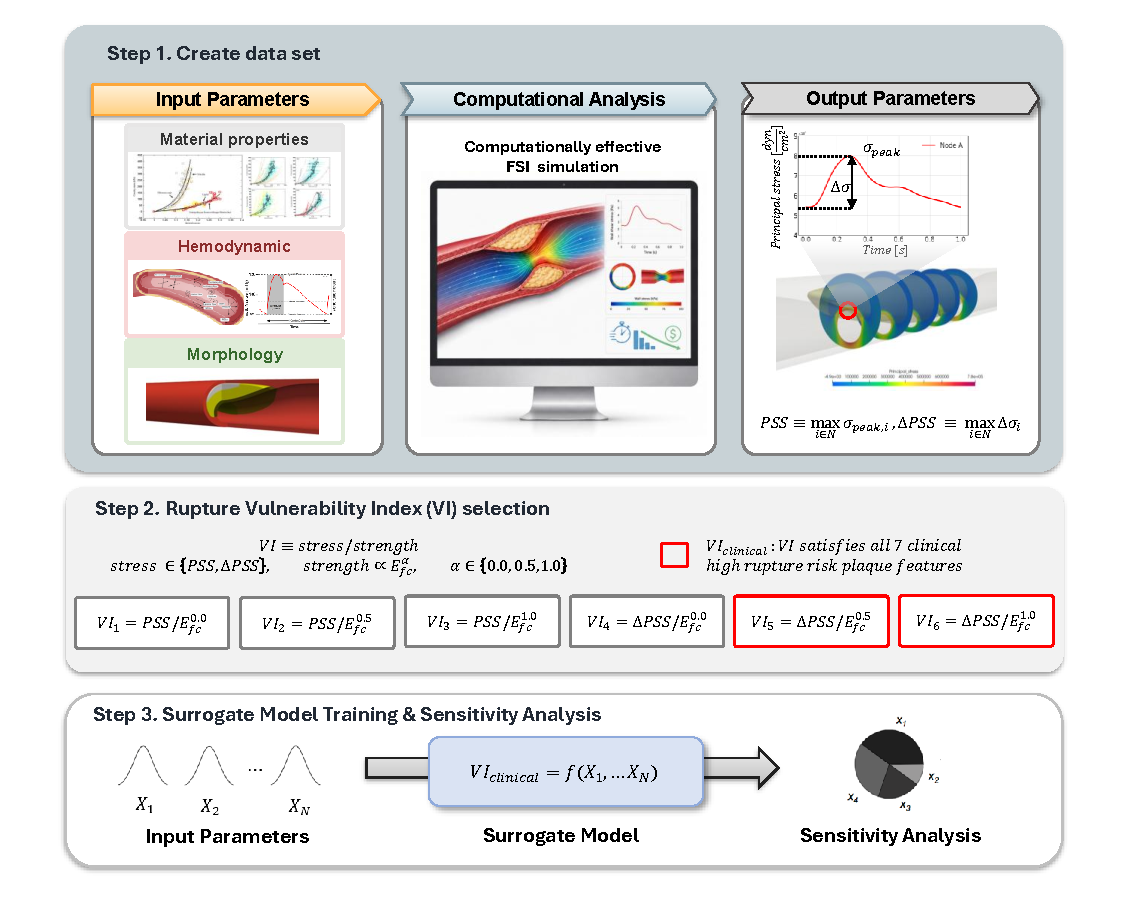
\includegraphics[width=\textwidth,height=0.82\textheight,keepaspectratio]{figures/figure_page_04.pdf}
\caption[Three-stage analysis workflow]{Overall workflow of the three-stage parametric analysis framework.}
\label{fig:ch3-workflow}
\end{figure}

\section{Data generation (Stage 1)}
As shown in Figure~\ref{fig:ch3-phenotype}, two high-risk plaque phenotypes frequently reported in coronary CT angiography (CCTA), LAP and CP, were modeled~\cite{lu2021highrisk, williams2020lap}. LAP was defined as a three-solid-domain model consisting of the vessel wall, fibrous cap (FC), and lipid core, whereas CP was defined as a four-solid-domain model with an additional calcification domain. The baseline coronary geometry was fixed as a cylindrical segment with a length of $10$~cm, lumen radius of $r_\mathrm{ref}=0.1$~cm, and wall thickness of $t_\mathrm{wall}=0.02$~cm~\cite{dodge1992lumen_r_av, fung1993biomechanics, caro2012mechanics}. The morphological input variables were defined under the premise that they could be derived from noninvasive and widely available CCTA, thereby facilitating future extension toward clinical application. Fibrous-cap thickness was not resolved by CCTA and can only be measured using invasive imaging modalities such as OCT~\cite{kume2005octimt}; therefore, it was assumed to be spatially uniform, reduced to a single scalar, and fixed at $t_\mathrm{FC} = 100\,\mu\mathrm{m}$, a representative value consistent with the in vivo OCT measurement range of vulnerable plaques, for all samples~\cite{jang2005oct}.

\begin{figure}[!htbp]
\centering
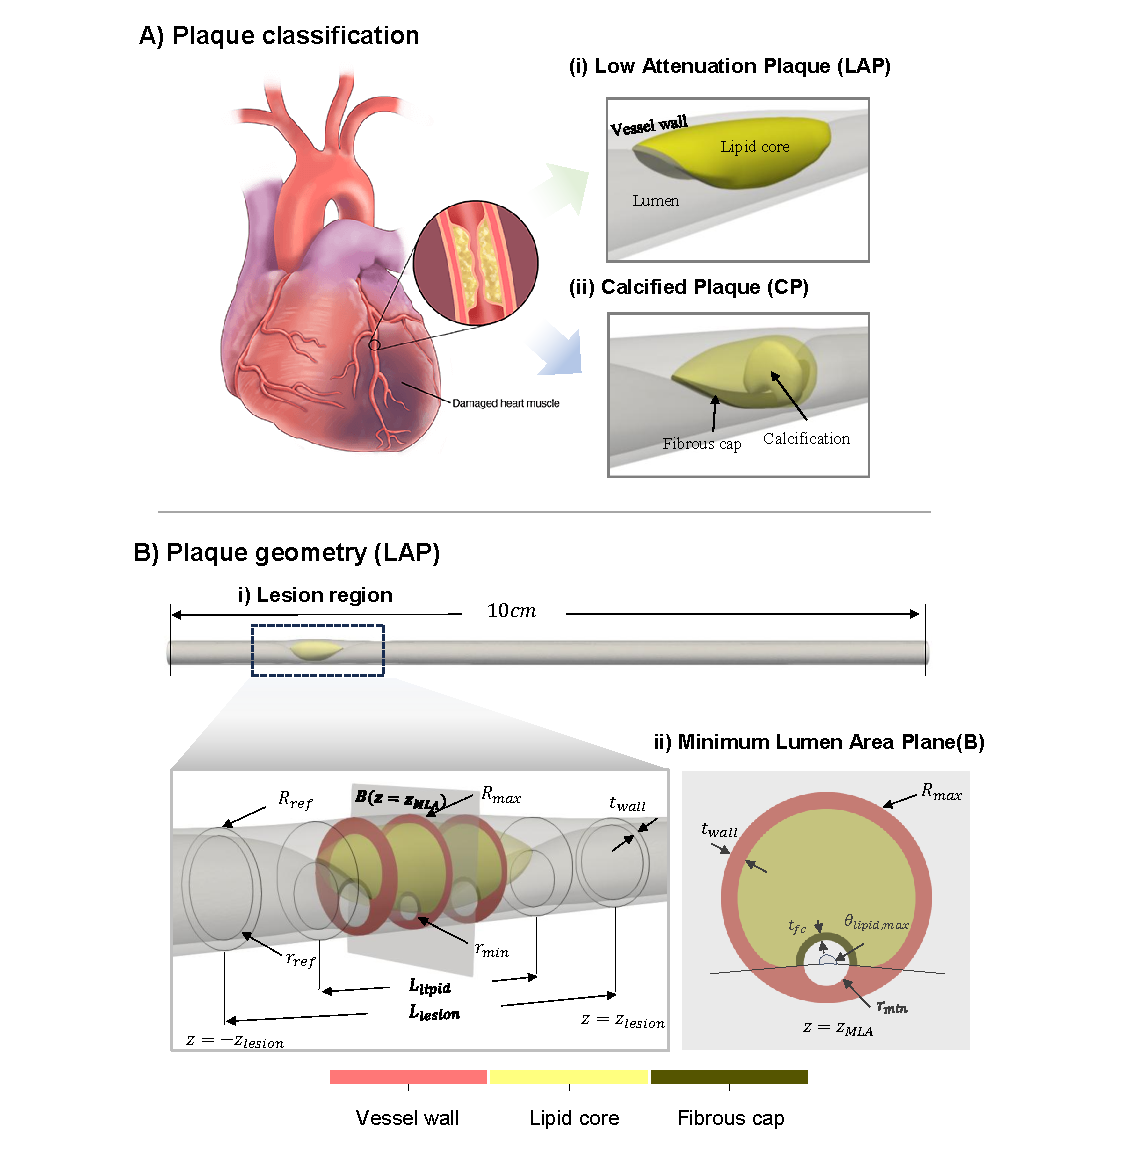
\includegraphics[width=\textwidth,height=0.82\textheight,keepaspectratio]{figures/figure_page_05.pdf}
\caption[Plaque phenotypes and morphological parameters]{Plaque phenotypes and morphological parameterization. (A) Two plaque phenotypes modeled in this study: low-attenuation plaque (LAP) and calcified plaque (CP). (B) Plaque geometry and clinically interpretable morphological parameters.}
\label{fig:ch3-phenotype}
\end{figure}

\subsection{Input parameters}
The input variables were composed of morphological, hemodynamic, and material factor groups. The morphological parameters were further divided into clinically interpretable analysis variables and auxiliary parameters for calcification-shape generation. Figure~\ref{fig:ch3-phenotype} illustrates the geometric meaning of the main morphological variables used for the LAP geometry, and the mathematical definitions, units, sampling ranges, and applicable plaque phenotypes of each variable are summarized in Table~\ref{tab:input-vars}. In this study, degree of stenosis $DS$, lesion length $L_\mathrm{lesion}$, lumen axial skewness $\gamma_z$, positive remodeling index $PI$, lipid arc angle $\theta_\mathrm{lipid,max}$, and lipid length ratio $l_\mathrm{lipid}$ were used as morphological input variables common to both LAP and CP. For the CP phenotype, calcified fraction $f_\mathrm{calc}$ was additionally included to represent calcification burden. Table~\ref{tab:input-vars} presents only clinically interpretable analysis variables, whereas the four auxiliary calcification-generation parameters used only during CP geometry generation are provided separately in Appendix~A.

Hemodynamic variables were defined as systolic pressure ($P_\mathrm{sys}$), pulse pressure ($\Delta P$), and diastolic decay ratio ($\tau$) to construct the pressure loading condition. Pulse pressure was defined as $\Delta P=P_\mathrm{sys}-P_\mathrm{dia}$, and the constraint $P_\mathrm{dia}>40\,\mathrm{mmHg}$ was imposed during sampling to exclude physiologically unrealistic low-pressure conditions~\cite{heward2025cpp, mcevoy2016diastolic}. Material variables were defined as the Young's modulus of each solid domain, and $E_\mathrm{calc}$ was additionally included as an input variable for calcified plaques. Coronary tissues were modeled as isotropic linear elastic materials under the assumption that they deform within a small-strain range during the cardiac cycle~\cite{milzi2021, loree1992}.

\begin{table}[ht]
\caption[Input variables]{Clinically interpretable analysis variables, definitions, units, and sampling ranges.}
\label{tab:input-vars}
\begin{center}
\small
\begin{tabular}{lllllc}
\hline\hline
Group & Variable & Symbol & Definition & Unit & Range [min, max] \\
\hline
Morphological & Degree of stenosis & $DS$ & $DS=(1-D_\mathrm{min}/D_\mathrm{ref})\times100$ & \% & [25, 75] \\
& Lesion length & $L_\mathrm{lesion}$ & --- & cm & [1.0, 3.0] \\
& Lumen axial skewness & $\gamma_z$ & $\gamma_z=z_\mathrm{MLA}/z_\mathrm{lesion}$ & --- & [$-0.75$, $0.75$] \\
& Positive remodeling index & $PI$ & $PI=A_\mathrm{max}/A_\mathrm{ref}$ & --- & [0.9, 1.2] \\
& Lipid arc angle & $\theta_\mathrm{lipid,max}$ & --- & deg & [120, 270] \\
& Lipid length ratio & $l_\mathrm{lipid}$ & $l_\mathrm{lipid}=L_\mathrm{lipid}/L_\mathrm{lesion}$ & --- & [0.5, 0.8] \\
& Calcified fraction (CP) & $f_\mathrm{calc}$ & $f_\mathrm{calc}=V_\mathrm{calc}/V_\mathrm{lesion}$ & --- & [0.20, 0.80] \\
Hemodynamic & Systolic pressure & $P_\mathrm{sys}$ & $P_\mathrm{sys}=\max_t P(t)$ & mmHg & [100, 170] \\
& Pulse pressure & $\Delta P$ & $\Delta P=P_\mathrm{sys}-P_\mathrm{dia}$ & mmHg & [35, 80] \\
& Decay ratio & $\tau$ & --- & --- & [0.01, 0.50] \\
Material & Vessel-wall modulus & $E_\mathrm{vessel}$ & --- & dyn/cm$^2$ & [$1\times10^6$, $1.4\times10^7$] \\
& Fibrous-cap modulus & $E_\mathrm{FC}$ & --- & dyn/cm$^2$ & [$4\times10^6$, $2.3\times10^7$] \\
& Lipid-core modulus & $E_\mathrm{lipid}$ & --- & dyn/cm$^2$ & [$1\times10^4$, $1\times10^6$] \\
& Calcification modulus (CP) & $E_\mathrm{calc}$ & --- & dyn/cm$^2$ & [$7\times10^9$, $2.5\times10^{11}$] \\
\hline\hline
\end{tabular}
\end{center}
\end{table}

The sampling ranges were selected based on values reported in previous clinical or imaging studies~\cite{ambrose1999, kang2018, vanvelzen2012, choi2015aps, lee2012remodeling, geng2021, wang2017plr, sugiura2021, ryan2021oct_lipid_review, krishnamoorthy2017, aha2024bp, danchin2004aorticpp, parenica2011aorticpp, westerhof2009windkessel, wangtang2021, holzapfel2005, karimi2013, loree1994static, teng2014material, cheng1993, barrett2019, cahalane2018, milzi2021}. The analysis variables summarized in Table~\ref{tab:input-vars} were then assumed to follow mutually independent uniform distributions within their respective ranges, and the input space was constructed using Latin hypercube sampling (LHS)~\cite{mckay1979lhs}.

For the LAP dataset, 1{,}000 input vectors were generated using the 12 analysis input variables listed in Table~\ref{tab:input-vars}. For the CP dataset, 1{,}000 input vectors were generated from an 18-dimensional LHS design consisting of the 14 analysis input variables in Table~\ref{tab:input-vars} and the four auxiliary calcification-generation parameters in Appendix~A. The auxiliary parameters were used to generate valid calcification geometries in the CP analysis, but they are not clinically directly interpretable plaque descriptors. Moreover, an initial Sobol screening analysis including all 18 variables was also performed~\cite{sobol1993sensitivity, saltelli2002sobol}, and the sensitivity contribution of the auxiliary parameters was confirmed to be negligible compared with those of the main morphological, hemodynamic, and material factors (numerical values are provided in Appendix~A). Accordingly, the final GPR model training and Sobol sensitivity analysis used only 14 clinically interpretable analysis input variables: the 12 variables common to LAP, with the addition of $f_\mathrm{calc}$ and $E_\mathrm{calc}$.

\subsection{Geometry and mesh}
For each LHS sample, a parametric CAD model was programmatically generated using Autodesk Inventor Professional 2026 (Autodesk Inc., San Francisco, CA, USA) and discretized into separate fluid and solid finite-element meshes. Calcification, used only for CP, was generated within the lipid core using a seed-based region-growing algorithm to reproduce irregular clinically observed morphologies; the full procedure is described in Appendix~A. The solid domains were discretized using second-order tetrahedral elements in the open-source software Gmsh~\cite{geuzaine2009gmsh}, with a box-meshing strategy near the lesion, resulting in approximately $3$--$4\times10^6$ elements per sample. The fluid domain was discretized using Simmetrix MeshSim (Simmetrix Inc., Clifton Park, NY, USA)~\cite{simmetrix_meshsim} with approximately $5.5\times10^6$ first-order tetrahedral elements and three prism boundary-layer layers along the lumen wall. Mesh independence was assessed by varying the representative element size in the lesion region to $0.05$, $0.04$, and $0.03$~cm and evaluating the maximum principal stress in the fibrous-cap domain. Because the results for $0.04$~cm and $0.03$~cm were nearly identical, with a relative difference of $<1\%$, $0.04$~cm was adopted for the final simulations.

\subsection{Boundary conditions}

\begin{figure}[!htbp]
\centering
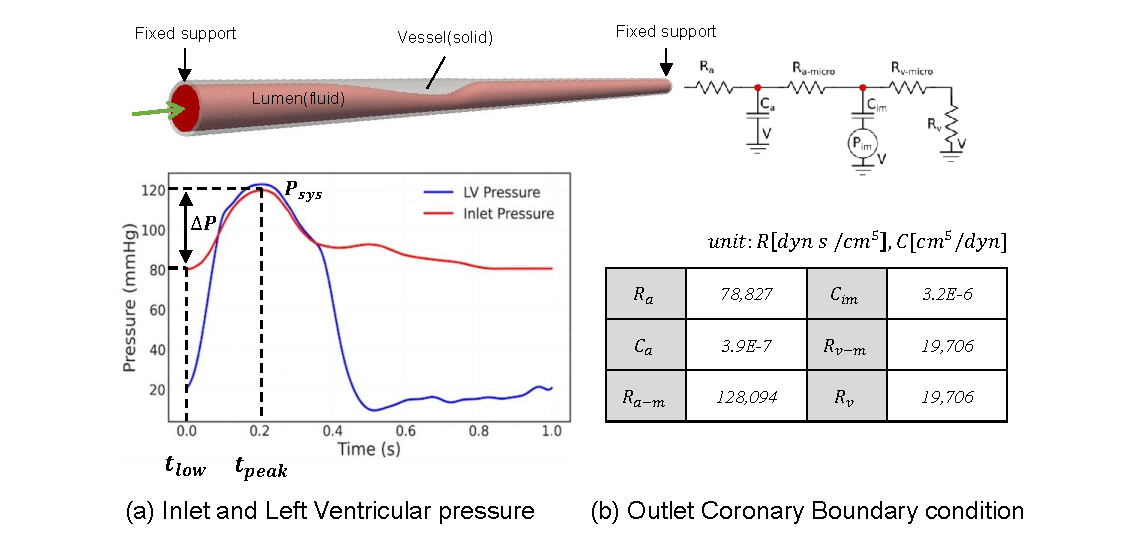
\includegraphics[width=\textwidth,height=0.82\textheight,keepaspectratio]{figures/figure_page_06.pdf}
\caption[Parametric model boundary conditions]{Boundary conditions for the fluid and solid analyses.}
\label{fig:ch3-bc}
\end{figure}

As the fluid boundary condition, a physiological pressure waveform $P_\mathrm{in}(t)$ was prescribed at the inlet. This pressure waveform was generated by coupling a fixed reference coronary flow waveform $Q(t)$ with a three-element Windkessel (RCR) model, and the remaining parameters were fitted by least squares while fixing the coronary resistance ratio at $R_p/R_d=1/10$~\cite{westerhof2009windkessel}. Thus, $P(t)$ for each sample was fully determined by the three hemodynamic variables $P_\mathrm{sys}$, $\Delta P$, and $\tau$; the detailed waveform-generation procedure is provided in Appendix~B.

At each outlet, a lumped-parameter coronary boundary condition was imposed to represent the distal coronary microvasculature~\cite{kim2010coronary}. First, the total distal resistance ($R_{\mathrm{tot},i}$) was calculated using the reference mean outlet flow rate (0.35~cc/s) and mean pressure (93.3~mmHg)~\cite{guyton2011_av_P}. Then, $R_{\mathrm{tot},i}$ was distributed among the resistance components constituting the coronary boundary condition according to predefined ratios, and the compliance component was set based on values reported in previous studies~\cite{Sankaran2012}. The final resistance and compliance parameters shown in Figure~\ref{fig:ch3-bc} were applied to each outlet. In addition, a time-varying intramyocardial pressure $P_{\mathrm{im}}(t)$ was imposed to account for myocardial compression in the coronary boundary condition. $P_{\mathrm{im}}(t)$ was calculated using a reduced-order heart-model ODE for the same cardiac phase as the inlet pressure waveform $P_{\mathrm{in}}(t)$, and the detailed equations and calculation procedure are provided in Appendix~B.

For the solid boundary condition, the wall pressure field reconstructed from the three-dimensional steady fluid simulation was applied as a surface traction on the inner wall of the multi-domain solid mesh, and both ends of the vascular segment were constrained as fixed ends.

\subsection{Output parameters}
The output parameters in this study consisted of stress-magnitude indices for each case and rupture location indices derived from the sites of peak stress. First, end-systole ($t_\mathrm{sys}$) and end-diastole ($t_\mathrm{dia}$) were extracted from the inlet pressure waveform, and computationally efficient FSI simulations were performed at both time points to compute the maximum principal stress distribution on the fibrous-cap surface. Plaque structural stress (PSS) for each case was then defined as the maximum value of the maximum principal stress occurring on the fibrous-cap surface at end-systole, and the pulsatile plaque structural stress amplitude ($\Delta\mathrm{PSS}$) was defined as the maximum change in maximum principal stress between end-systole and end-diastole~\cite{gu2022, huang2021dpss, costopoulos2017}:

\begin{equation}
\mathrm{PSS} = \max_{n\,\in\,\Gamma_\mathrm{fc}} \sigma_n(t_\mathrm{sys}), \qquad \Delta\mathrm{PSS} = \max_{n\,\in\,\Gamma_\mathrm{fc}} \left[\sigma_n(t_\mathrm{sys}) - \sigma_n(t_\mathrm{dia})\right]
\end{equation}

Here, $\Gamma_\mathrm{fc}$ denotes the set of fibrous-cap surface nodes. PSS corresponds to the systolic maximum principal stress for a monotonic failure scenario, whereas $\Delta$PSS corresponds to the pulsatile stress amplitude for a fatigue failure scenario. To reduce single-node noise, $\sigma_n$ at each node was spatially averaged within a spherical neighborhood of radius $r=0.01$~cm before calculating the maximum value~\cite{corti2022}.

The location of each predicted rupture node was then quantified in the axial and circumferential directions. The axial rupture location was classified into proximal, mid, and distal regions. The lumen area ratio at each axial location was defined as $LA(z)=A_\mathrm{lumen}(z)/A_\mathrm{normal}$, and, following the lesion-region definition of Chung et al.~\cite{chung2017_LA}, the two locations at which $LA=0.3$ were used as the proximal and distal boundaries of the mid region. As shown in Figure~\ref{fig:ch3-rupture}, a predicted rupture node located upstream of these two boundaries was classified as proximal, one located between the two boundaries as mid, and one located downstream as distal. The circumferential rupture location was calculated on the cross-section containing the predicted rupture node, referred to as the rupture plane. On this cross-section, $\theta_\mathrm{rupture}$ was defined as the angle between the reference $y$-axis and the vector connecting the lumen center to the predicted rupture node, and this angle was normalized by the lipid arc angle $\theta_\mathrm{lipid}$ on the same cross-section:

\begin{equation}
I_\theta=\frac{|\theta_\mathrm{rupture}|}{\theta_\mathrm{lipid}}
\end{equation}

Here, $I_\theta=0$ indicates a location close to the cap center, whereas $I_\theta=1$ indicates a location close to the plaque shoulder. Therefore, the final output parameters of this study consisted of the maximum PSS, maximum $\Delta\mathrm{PSS}$, axial rupture location, and circumferential rupture location index for each case.

\begin{figure}[!htbp]
\centering
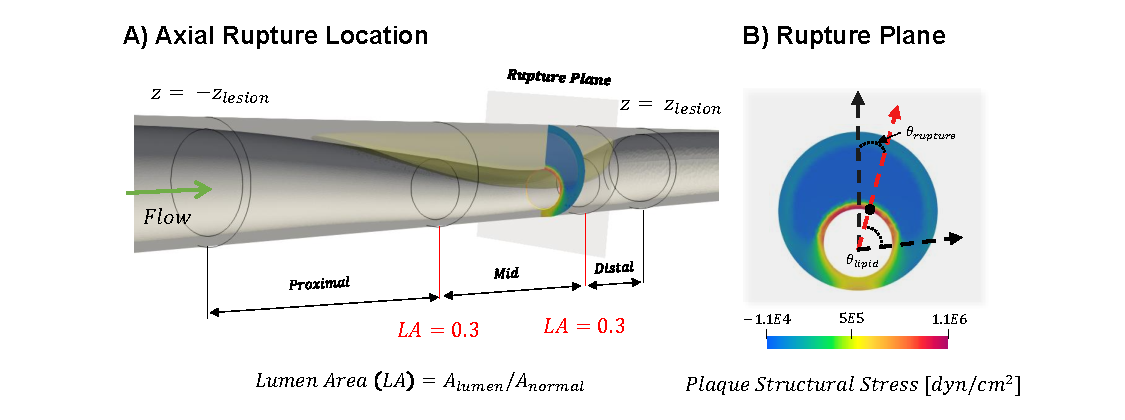
\includegraphics[width=\textwidth,height=0.82\textheight,keepaspectratio]{figures/figure_page_07.pdf}
\caption[Rupture location index definition]{Definition of axial and circumferential rupture location indices.}
\label{fig:ch3-rupture}
\end{figure}

\section{Vulnerability index formulation and selection (Stage 2)}
\subsection{VI formulation}
Because rupture occurs when stress exceeds strength, the vulnerability index was defined as the ratio of stress to strength: $\mathrm{VI}=\mathrm{stress}/\mathrm{strength}$~\cite{corti2022}. In this formulation, the stress term was represented by either PSS or $\Delta$PSS. Although previous plaque-rupture models have commonly treated fibrous-cap strength as a fixed ultimate-stress threshold~\cite{ohayon2008, corti2022, dolla2012, kok2016}, its dependence on material stiffness remains uncertain. Therefore, three rupture scenarios---fixed ultimate stress, energy density, and fixed ultimate strain---were combined with the isotropic linear elastic assumption to parameterize strength using a single exponent $\alpha$. Each exponent corresponds to a classical failure theory: $\alpha=0$ to Rankine theory (maximum stress), $\alpha=0.5$ to Beltrami theory (energy density), and $\alpha=1$ to St.~Venant theory (maximum strain)~\cite{ugural2003advanced}. By combining the two stress measures with the three strength exponents, six candidate VIs were defined for each case:

\begin{equation}
\mathrm{strength} \propto E_\mathrm{FC}^{\alpha}, \qquad \mathrm{VI}(\sigma,\alpha) = \frac{\sigma}{E_\mathrm{FC}^{\alpha}}, \qquad \sigma\in\{\mathrm{PSS},\Delta\mathrm{PSS}\},\ \alpha\in\{0.0,\ 0.5,\ 1.0\}
\end{equation}

\subsection{VI candidate selection (seven-criterion rubric)}
To identify physically plausible indices among the six VI candidates defined above, clinically recognized high-risk plaque features were used as an evaluation rubric. Specifically, seven plaque features widely recognized in the medical literature as being associated with high rupture risk were reviewed, and each feature was translated into a model-measurable feature and the expected direction of correlation with vulnerability, as summarized in Table~\ref{tab:seven-criteria}. For example, a soft plaque substrate was translated into low $E_\mathrm{lipid}$ and an expected negative correlation with vulnerability.

Five of the seven criteria were directly represented by input variables ($E_\mathrm{lipid}$, $f_\mathrm{calc}$, $\theta_\mathrm{lipid}$, $E_\mathrm{FC}$, and $t_\mathrm{FC}$), whereas plaque burden (criterion 4) and $\Delta\mathrm{FFR}$ (criterion 5) were not prescribed inputs but were instead derived from the plaque geometry and simulation results. Plaque burden generally refers to the amount of atherosclerotic plaque within the vessel wall and is commonly quantified from plaque area or volume~\cite{mintz2001ivus}. In this study, plaque burden was not intended to reproduce the clinical plaque-burden measurement directly; instead, it was used as a model-level operational measure of the low-attenuation plaque component and was defined as the volume of the lipid-core domain~\cite{williams2020lap}.

$\Delta\mathrm{FFR}$ was used as a model-level FFR-derived index to quantify the normalized pressure loss induced by the lesion. FFR is generally defined as the ratio of distal coronary pressure $P_d$ to proximal, or aortic, pressure $P_a$, i.e., $\mathrm{FFR}=P_d/P_a$. In this study, $\Delta\mathrm{FFR}$ was defined as the difference between proximal and distal FFR: $\Delta\mathrm{FFR} = \mathrm{FFR}_\mathrm{proximal} - \mathrm{FFR}_\mathrm{distal}$~\cite{lee2019emerald}. Under the idealized inlet condition, $P_a=P_\mathrm{in}$ and thus $\mathrm{FFR}_\mathrm{proximal}=1$, so $\Delta\mathrm{FFR}=1-P_d/P_\mathrm{in}$. Here, $P_d$ was calculated as the cross-sectional mean pressure $3\,\mathrm{cm}$ downstream of the lesion~\cite{cami2018ffrct}. Thus, $\Delta\mathrm{FFR}$ was used as a model-level surrogate of the lesion-level functional gradient, rather than as a direct reproduction of clinical FFR.

A valid VI was expected to vary consistently with the seven high-risk features in the clinically expected directions. Because the absolute fibrous-cap strength was not directly known, magnitude-based validation was not possible. Therefore, for each candidate--criterion pair, only the sign of the Spearman rank correlation between the corresponding feature and VI was compared with the expected direction defined \emph{a priori} from clinical evidence. If the sign agreed with the expected direction, the candidate was classified as compliant (\checkmark); otherwise, it was classified as non-compliant ($\times$). Only candidates satisfying all seven criteria were regarded as physically admissible, whereas any VI showing an opposite direction for at least one criterion was excluded.

\begin{table}[ht]
\caption[Seven high-risk plaque features]{Seven established high-risk plaque features used for VI selection.}
\label{tab:seven-criteria}
\begin{center}
\begin{tabular}{clllc}
\hline\hline
\# & Clinical fact & Model feature & Expected sign & Data \\
\hline
1 & Soft plaque substrate & Low $E_\mathrm{lipid}$ & $-$ & LAP \\
2 & Less calcified plaque fraction & Low $f_\mathrm{calc}$ & $-$ & CP \\
3 & Large lipid arc angle & Large $\theta_\mathrm{lipid}$ & $+$ & LAP \\
4 & Large plaque burden & High model-level plaque burden & $+$ & LAP \\
5 & Functional gradient & High $\Delta$FFR & $+$ & LAP \\
6 & Collagen-deficient fibrous cap & Low $E_\mathrm{FC}$ & $-$ & LAP \\
7 & Thin fibrous cap & Low fibrous-cap thickness & $-$ & * \\
\hline\hline
\end{tabular}\\
*: additional 15-simulation data. References: \cite{motoyama2009, liu2025calc, prati2020clima, xing2017, williams2020lap, erlinge2021prospect2, takagi2022dffrct, lee2019emerald, sukhova1999, savvopoulos2024afm, stone2011prospect, naghavi2003vulnerable, virmani2006}.
\end{center}
\end{table}

Since criterion 7, fibrous-cap thickness, could not be evaluated using the baseline dataset in which $t_\mathrm{FC}$ was fixed, an auxiliary $5 \times 3$ parametric set was generated. In this set, $t_\mathrm{FC}$ was varied from $4$ to $20~\mu\mathrm{m}$ in increments of $4~\mu\mathrm{m}$, and $E_\mathrm{FC}$ was varied over $1.2$, $1.6$, and $2.0~\mathrm{MPa}$, while all remaining input parameters were fixed at the midpoints of their prescribed ranges.

\section{Surrogate-based global sensitivity analysis (Stage 3)}
The objective of this stage was to quantify the sensitivity of plaque rupture risk to morphological, hemodynamic, and material factors. Because Sobol sensitivity analysis requires more than 10{,}000 model evaluations per phenotype, direct application to the FSI model was computationally infeasible even with the cost-effective FSI framework. Therefore, a Gaussian process regression (GPR) surrogate model was first trained to learn the input-to-VI mapping, and Sobol variance-based global sensitivity analysis was then performed on the surrogate.

\subsection{GPR surrogate model}
For each VI candidate and phenotype, an individual GPR surrogate model was trained to map the input vector ($d=12$ for LAP and $d=14$ for CP) to a scalar VI. After excluding samples that failed during geometry generation, including Boolean operations, or meshing, the valid sample sizes were $784/1{,}000$ for LAP and $756/1{,}000$ for CP. The valid samples were randomly divided into training and test sets at an $8\!:\!2$ ratio. The model was implemented using \texttt{GaussianProcessRegressor} in scikit-learn~\cite{pedregosa2011scikit}, with a squared-exponential kernel using automatic relevance determination (ARD), i.e., separate length-scale parameters for each input dimension~\cite{rasmussen2006gpml}. Kernel hyperparameters were determined by maximizing the marginal log-likelihood. Predictive accuracy was reported as the coefficient of determination ($R^2$) on the held-out test set.

\subsection{Sobol variance-based indices}
Sobol variance-based global sensitivity analysis was performed using the trained GPR surrogate models~\cite{sobol2001global, saltelli2002sobol, saltelli2010variance}. Here, $Y$ denotes the representative VI predicted by the GPR surrogate, $X_i$ denotes the $i$-th input variable, $X_{\sim i}$ denotes all input variables except $X_i$, and $X_G$ denotes the set of variables belonging to factor group $G$. The first-order index $S_i$ quantifies the individual contribution of $X_i$ to the output variance, whereas the total-order index $S_{Ti}$ quantifies its total contribution, including interaction effects:

\begin{equation}
S_i = \frac{\mathrm{Var}_{X_i}\!\left[\mathbb{E}_{X_{\sim i}}(Y\mid X_i)\right]}{\mathrm{Var}(Y)}, \qquad S_{Ti} = \frac{\mathbb{E}_{X_{\sim i}}\!\left[\mathrm{Var}_{X_i}(Y\mid X_{\sim i})\right]}{\mathrm{Var}(Y)}
\end{equation}

First-order and total-order indices were estimated using the Saltelli sampling scheme based on Sobol quasi-random sequences~\cite{saltelli2002sobol, saltelli2010variance}. With a base sample size of $N=1{,}024$, this required $N(d+2)$ surrogate evaluations: 14{,}336 evaluations for LAP ($d=12$) and 16{,}384 evaluations for CP ($d=14$). In addition to individual-variable indices, group-level Sobol indices $S_G$ and $S_{TG}$ were calculated for the three factor groups $G\in\{\mathrm{morphological, material, hemodynamic}\}$. These group-level indices were computed by treating each factor group as a grouped input, rather than by summing individual-variable indices, thereby accounting for interactions among variables within each group~\cite{saltelli2008}:

\begin{equation}
S_G = \frac{\mathrm{Var}_{X_G}\!\left[\mathbb{E}_{X_{\sim G}}(Y\mid X_G)\right]}{\mathrm{Var}(Y)}, \qquad S_{TG} = \frac{\mathbb{E}_{X_{\sim G}}\!\left[\mathrm{Var}_{X_G}(Y\mid X_{\sim G})\right]}{\mathrm{Var}(Y)}
\end{equation}


%%======================================================================
%% Chapter 4. Results
%%======================================================================
\chapter{Results}

This chapter presents the results of the three-stage framework for the two plaque phenotypes, LAP and CP. First, the simulated outputs were compared with clinical and computational studies to assess their literature-based consistency (\S4.1). Six vulnerability index candidates were then screened based on clinical criteria, and two final indices were selected (\S4.2). The Sobol global sensitivity analysis results for these indices are presented next (\S4.3).

\section{Simulated stress, FFR, and rupture-location results}

\begin{figure}[!htbp]
\centering
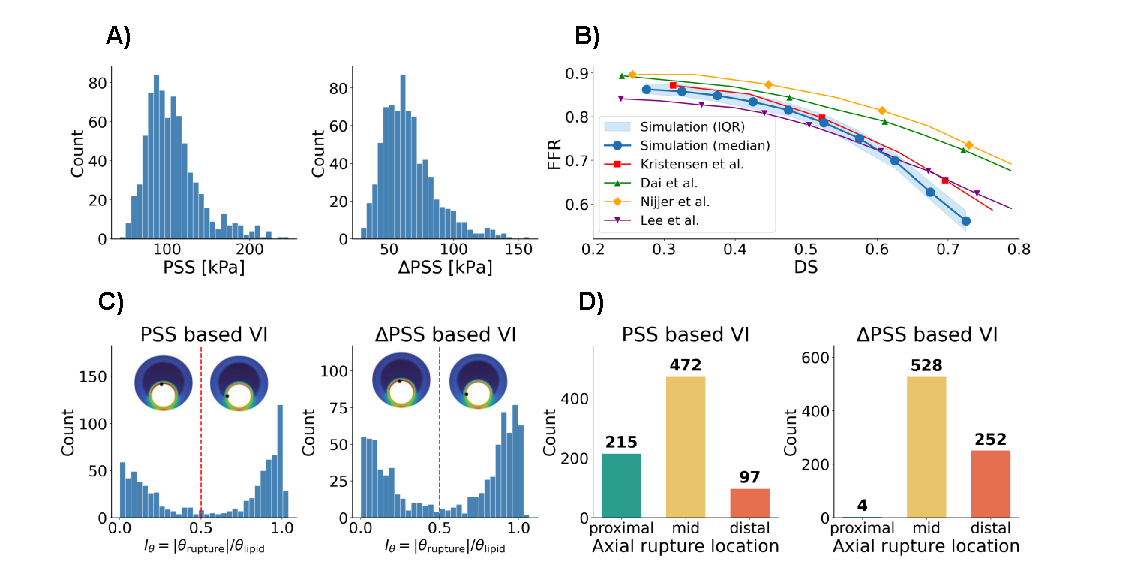
\includegraphics[width=\textwidth,height=0.82\textheight,keepaspectratio]{figures/figure_page_08.pdf}
\caption[Simulated stress, FFR, and rupture locations]{Simulated stress, FFR, and rupture-location results. (A) Distributions of simulated $\mathrm{PSS}$ and $\Delta\mathrm{PSS}$ in the LAP dataset. (B) Simulated FFR--DS relationship in the LAP dataset. (C,D) Circumferential and axial distributions of predicted rupture locations in the LAP dataset.}
\label{fig:res-sim}
\end{figure}

Before VI screening, the simulated stress, FFR, and rupture-location outputs were examined in the LAP dataset (Fig.~\ref{fig:res-sim}). The simulated PSS values ranged from 43 to 247~kPa, with a median of 101~kPa and an interquartile range of 84--121~kPa. The 5th--95th percentile range was 65--174~kPa. The simulated $\Delta\mathrm{PSS}$ values ranged from 28 to 158~kPa, with a median of 62~kPa and an interquartile range of 51--76~kPa (Fig.~\ref{fig:res-sim}A). Moreover, the simulated FFR decreased as DS increased (Fig.~\ref{fig:res-sim}B). The median FFR values were 0.86, 0.85, 0.80, 0.72, and 0.60 at DS values of 0.3, 0.4, 0.5, 0.6, and 0.7, respectively. This decreasing trend indicates that the simulated pressure-drop response increased with stenosis severity.

Predicted rupture locations were analyzed in the circumferential and axial directions. In the circumferential direction, rupture was more frequently predicted at the shoulder than at the center. For the PSS-based VI, 338 cases (43.1\%) were located at the center and 446 cases (56.9\%) at the shoulder. For the $\Delta\mathrm{PSS}$-based VI, 333 cases (42.5\%) were located at the center and 451 cases (57.5\%) at the shoulder (Fig.~\ref{fig:res-sim}C). In the axial direction, rupture was concentrated in the middle region near the minimum lumen area. For the PSS-based VI, the proximal, middle, and distal regions accounted for 215 (27.4\%), 472 (60.2\%), and 97 cases (12.4\%), respectively. For the $\Delta\mathrm{PSS}$-based VI, the corresponding numbers were 4 (0.5\%), 528 (67.3\%), and 252 cases (32.1\%) (Fig.~\ref{fig:res-sim}D).

\section{Selection of vulnerability indices}
As defined in \S3, this study constructed six VI candidates by combining the stress term (PSS or $\Delta$PSS) with the fibrous-cap material strength term ($E_\mathrm{FC}^{\alpha}$, $\alpha=0.0/0.5/1.0$). In this section, each candidate was evaluated according to whether it showed correlations in directions consistent with seven clinically established high-risk plaque features, defined in Table~\ref{tab:seven-criteria}, and the final vulnerability indices were selected accordingly. A candidate was considered an admissible index only when its correlation sign matched the expected direction for all high-risk features.

\begin{figure}[!htbp]
\centering
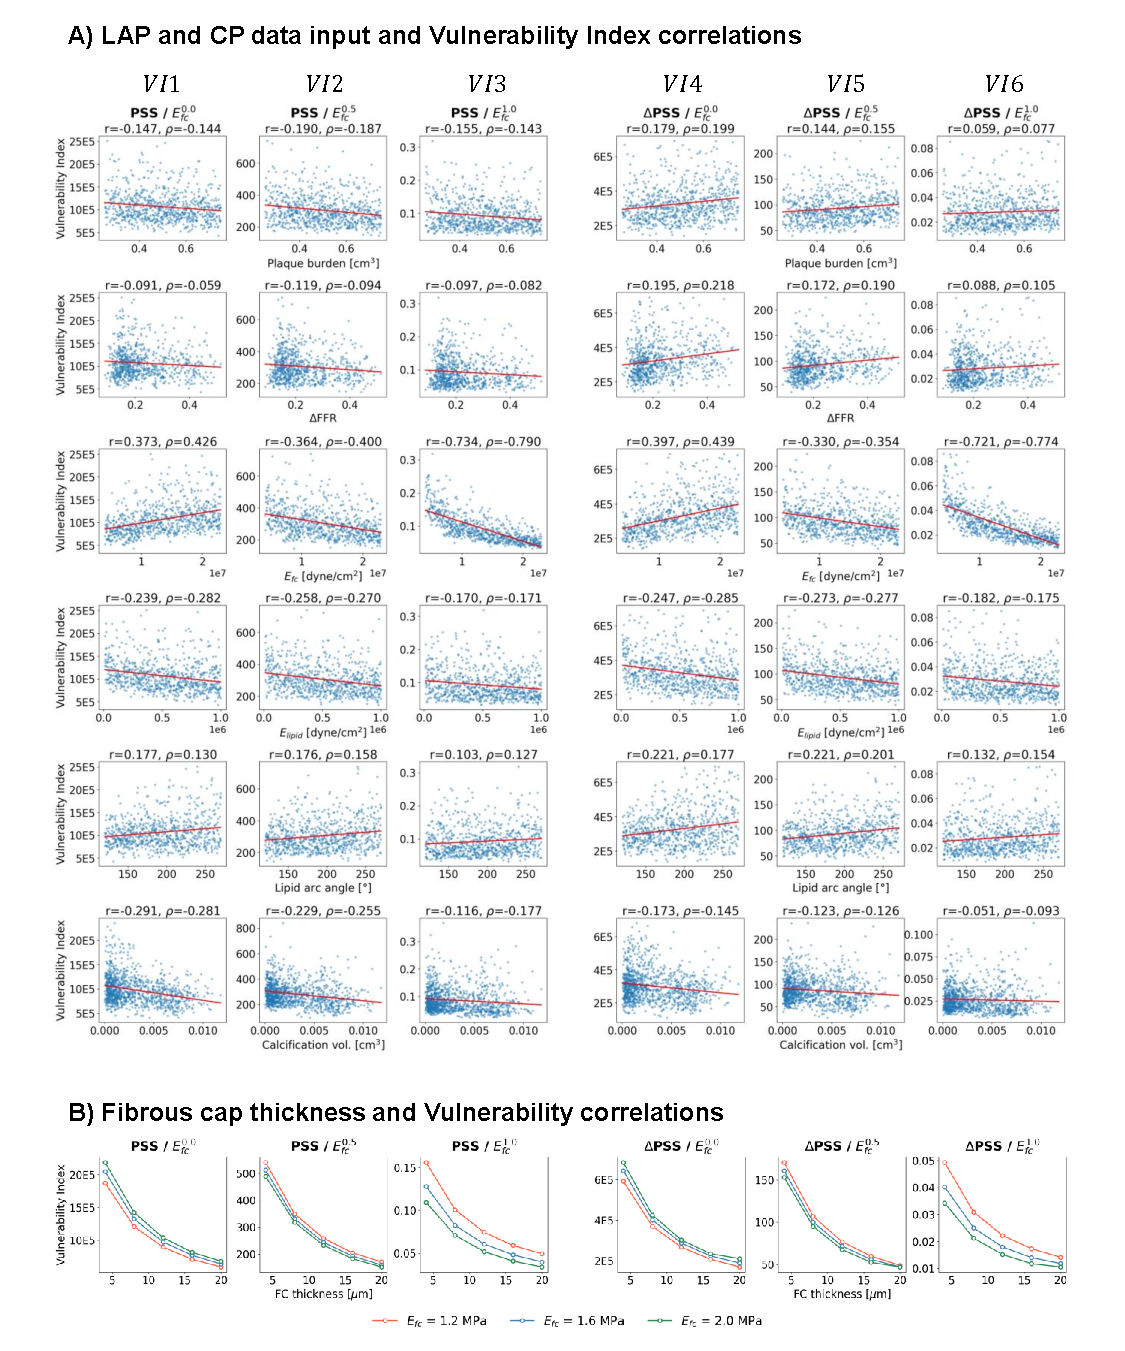
\includegraphics[width=\textwidth,height=0.82\textheight,keepaspectratio]{figures/figure_page_09.pdf}
\caption[VI candidate screening]{Correlation-based screening of vulnerability index candidates. (A) Input--VI correlations for six high-risk plaque features evaluated using the baseline LAP and CP datasets. (B) Fibrous-cap thickness--VI correlations evaluated using an auxiliary parametric dataset in which $t_\mathrm{FC}$ and $E_\mathrm{FC}$ were varied.}
\label{fig:res-screen}
\end{figure}

Pearson's correlation coefficient $r$ and Spearman's rank correlation coefficient $\rho$ were computed for each feature--VI candidate pair. Among the seven features, soft plaque, large lipid arc angle, less calcified plaque, and thin fibrous cap showed clinically expected correlation signs for all six candidates. Thus, for these features, all candidates satisfied clinical consistency and therefore did not serve as discriminating criteria among candidates. In contrast, the correlation sign differed across candidates for plaque burden, $\Delta$FFR, and $E_\mathrm{FC}$, and these three features served as the key criteria for selecting the final VI candidates. The expected correlation direction for each feature and whether each of the six VI candidates satisfied that direction are summarized in Table~\ref{tab:vi-compliance}.

\begin{table}[ht]
\caption[VI compliance matrix]{VI compliance matrix. Expected correlation direction between high-risk plaque features and VI, and compliance of the six VI candidates. \checkmark: clinically consistent; $\times$: violates expected direction.}
\label{tab:vi-compliance}
\begin{center}
\small
\begin{tabular}{clcccccccc}
\hline\hline
\# & High-risk feature & Param. & Exp. & PSS/$E^{0.0}$ & PSS/$E^{0.5}$ & PSS/$E^{1.0}$ & $\Delta$PSS/$E^{0.0}$ & $\Delta$PSS/$E^{0.5}$ & $\Delta$PSS/$E^{1.0}$ \\
\hline
1 & Large plaque burden & Plaque burden & $+$ & $\times$ & $\times$ & $\times$ & \checkmark & \checkmark & \checkmark \\
2 & High $\Delta$FFR & $\Delta$FFR & $+$ & $\times$ & $\times$ & $\times$ & \checkmark & \checkmark & \checkmark \\
3 & Collagen-deficient cap & $E_\mathrm{FC}$ & $-$ & $\times$ & \checkmark & \checkmark & $\times$ & \checkmark & \checkmark \\
4 & Soft plaque & $E_\mathrm{lipid}$ & $-$ & \checkmark & \checkmark & \checkmark & \checkmark & \checkmark & \checkmark \\
5 & Large lipid arc angle & $\theta_\mathrm{lipid,max}$ & $+$ & \checkmark & \checkmark & \checkmark & \checkmark & \checkmark & \checkmark \\
6 & Less calcified plaque & $V_\mathrm{calc}$ & $-$ & \checkmark & \checkmark & \checkmark & \checkmark & \checkmark & \checkmark \\
7 & Thin fibrous cap & $t_\mathrm{fc}$ & $-$ & \checkmark & \checkmark & \checkmark & \checkmark & \checkmark & \checkmark \\
\hline
\multicolumn{4}{c}{\textbf{All 7 satisfied?}} & $\times$ & $\times$ & $\times$ & $\times$ & \textbf{\checkmark} & \textbf{\checkmark} \\
\hline\hline
\end{tabular}
\end{center}
\end{table}

As a result, among the six candidates, only $\Delta$PSS/$E_\mathrm{FC}^{0.5}$ and $\Delta$PSS/$E_\mathrm{FC}^{1.0}$ satisfied all criteria. The PSS-based candidates did not satisfy the clinically expected directions for plaque burden and $\Delta$FFR, regardless of the value of $\alpha$. Specifically, plaque risk would be expected to increase as plaque burden and $\Delta$FFR increase, but the PSS-based VI showed weak negative correlations with these features ($\rho \approx -0.143, -0.144, -0.187$). In contrast, for the same features, the $\Delta$PSS-based VI showed positive correlations ($\rho \approx +0.199, +0.155, +0.077$), corresponding to the expected direction. This indicates that the pulsatile stress amplitude during the cardiac cycle reflects high-risk plaque features more consistently than the peak systolic stress at a single time point.

In addition, the $\alpha=0.0$ candidate without strength normalization did not satisfy the collagen-deficient (low $E_\mathrm{FC}$) cap criterion. In this case, a positive correlation ($\rho \approx +0.373, +0.397$) was observed between VI and $E_\mathrm{FC}$, which was opposite to the clinical expectation that reduced fibrous-cap material strength is associated with increased vulnerability. In contrast, for candidates with $E_\mathrm{FC}^{\alpha}$ included in the denominator ($\alpha \geq 0.5$), the correlation between VI and $E_\mathrm{FC}$ shifted to the negative direction ($\rho \approx -0.33$ to $-0.79$).

Therefore, based on directional consistency with clinically high-risk plaque features, this study adopted $\Delta$PSS/$E_\mathrm{FC}^{0.5}$ and $\Delta$PSS/$E_\mathrm{FC}^{1.0}$ as the final vulnerability indices, denoted as $\mathrm{VI}_5$ and $\mathrm{VI}_6$, respectively.

\section{Sensitivity analysis results}
\subsection{Accuracy of the GPR surrogate models}
For the two selected vulnerability indices, $\mathrm{VI}_5\ (\Delta\mathrm{PSS}/E_\mathrm{FC}^{0.5})$ and $\mathrm{VI}_6\ (\Delta\mathrm{PSS}/E_\mathrm{FC}^{1.0})$, GPR surrogate models were constructed to approximate the relationship between the input parameters and VI for each phenotype (LAP and CP). The numbers of valid input--output pairs were 784 for LAP and 756 for CP, and the leave-one-out cross-validation coefficients of determination ($R^2$) for each model are presented in Table~\ref{tab:gpr-accuracy}. After sufficient predictive accuracy was confirmed in all four GPR models, they were considered suitable surrogate models for the subsequent Sobol sensitivity analysis.

\begin{table}[ht]
\caption[GPR surrogate accuracy]{Accuracy of GPR surrogate models.}
\label{tab:gpr-accuracy}
\begin{center}
\begin{tabular}{llcc}
\hline\hline
Phenotype & Target VI & Valid samples & $R^2$ \\
\hline
LAP & $\mathrm{VI}_5$: $\Delta$PSS/$E_\mathrm{FC}^{0.5}$ & 784 & 0.93 \\
LAP & $\mathrm{VI}_6$: $\Delta$PSS/$E_\mathrm{FC}^{1.0}$ & 784 & 0.97 \\
CP  & $\mathrm{VI}_5$: $\Delta$PSS/$E_\mathrm{FC}^{0.5}$ & 756 & 0.92 \\
CP  & $\mathrm{VI}_6$: $\Delta$PSS/$E_\mathrm{FC}^{1.0}$ & 756 & 0.95 \\
\hline\hline
\end{tabular}
\end{center}
\end{table}

\subsection{Sobol global sensitivity indices}

\begin{figure}[!htbp]
\centering
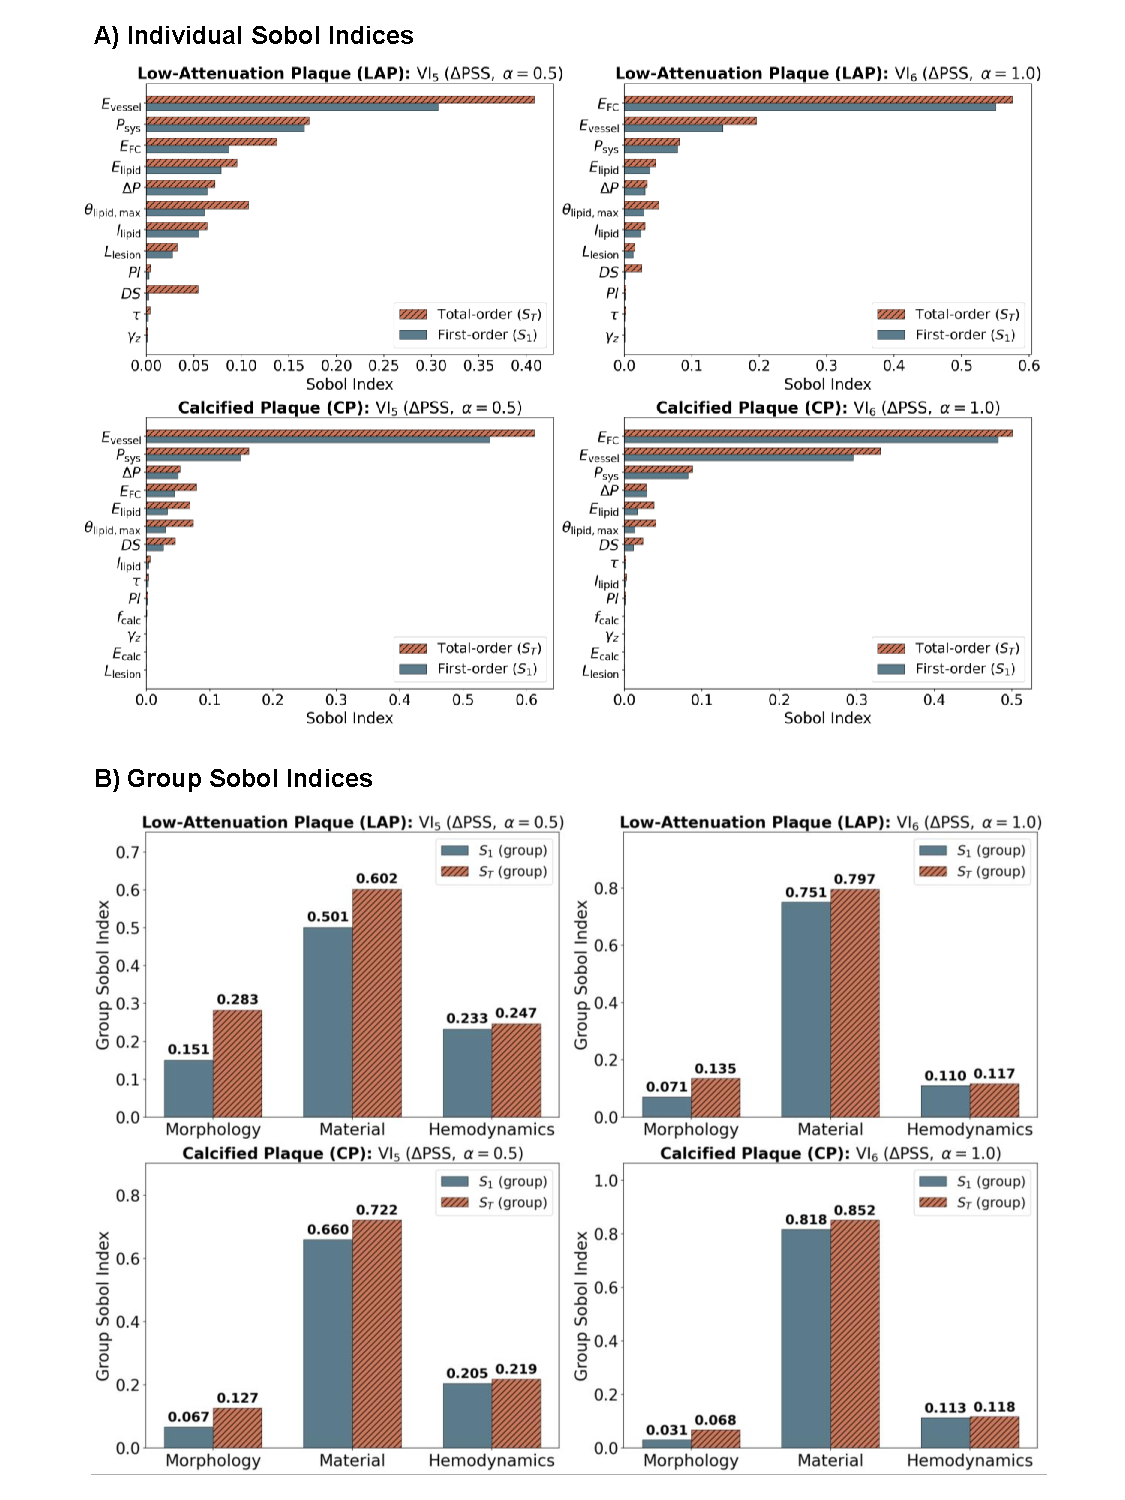
\includegraphics[width=\textwidth,height=0.82\textheight,keepaspectratio]{figures/figure_page_10.pdf}
\caption[Sobol sensitivity analysis]{Sobol sensitivity analysis of the selected vulnerability indices. (A) Individual-variable first-order and total-order Sobol indices. (B) Group-level Sobol indices for morphology, material, and hemodynamic factors.}
\label{fig:res-sobol}
\end{figure}

Saltelli sampling was performed on the GPR surrogate models to compute the first-order index ($S_1$) and total-order index ($S_T$). At the individual-variable level in Fig.~\ref{fig:res-sobol}A, $E_\mathrm{vessel}$, $E_\mathrm{FC}$, and $P_\mathrm{sys}$ were among the dominant contributors across the four phenotype--VI combinations. For LAP with $\mathrm{VI}_5$, $E_\mathrm{vessel}$ showed the largest total-order index ($S_T = 0.408$), followed by $P_\mathrm{sys}$ ($S_T = 0.171$) and $E_\mathrm{FC}$ ($S_T = 0.137$). For LAP with $\mathrm{VI}_6$, the ranking shifted: $E_\mathrm{FC}$ became the most influential variable ($S_T = 0.575$), followed by $E_\mathrm{vessel}$ ($S_T = 0.196$) and $P_\mathrm{sys}$ ($S_T = 0.081$). Similarly, for CP with $\mathrm{VI}_5$, $E_\mathrm{vessel}$ exhibited the highest sensitivity ($S_T = 0.612$), while for CP with $\mathrm{VI}_6$, $E_\mathrm{FC}$ again led ($S_T = 0.501$), followed by $E_\mathrm{vessel}$ ($S_T = 0.331$). These results indicate that VI variability was mainly governed by material stiffness properties and systolic pressure. In contrast, the morphological variables showed relatively low individual $S_1$ values, but several variables exhibited $S_T$ values notably larger than $S_1$, suggesting that they influenced VI through interactions with other inputs. For example, the lipid arc angle ($\theta_\mathrm{lipid,max}$) in LAP with $\mathrm{VI}_5$ had $S_1 = 0.061$ versus $S_T = 0.107$, and the degree of stenosis ($DS$) showed $S_1 = 0.002$ versus $S_T = 0.054$, indicating substantial interaction contributions.

The same trend was observed in the group sensitivity results in Fig.~\ref{fig:res-sobol}B. The material group showed the largest $S_T$ across LAP and CP and across $\mathrm{VI}_5$ and $\mathrm{VI}_6$ ($S_T = 0.602$--$0.852$), followed by the hemodynamic group ($S_T = 0.117$--$0.247$). The morphology group showed the lowest first-order contribution ($S_1 = 0.031$--$0.151$), but its $S_T$ ranged from 0.068 to 0.283, indicating a tendency to contribute to VI through interaction effects rather than through main effects alone.


%%======================================================================
%% Chapter 5. Discussion
%%======================================================================
\chapter{Discussion}

There are three main findings of this study. All admissible VIs that passed the clinical-consistency filter were based on $\Delta$PSS, the histologically expected direction was restored only when strength was normalized by $E_\mathrm{FC}^{\alpha}$ ($\alpha>0$) rather than treated as a constant ultimate stress, and material and hemodynamic factors dominated the sensitivity hierarchy. Before interpreting these findings, we first verify that the simulated dataset reproduces the prior observations.

\section{Verification of simulated outputs against clinical and computational evidence}
The simulated outputs in \S4.1 showed literature-based consistency with prior clinical and computational observations. As shown in Fig.~\ref{fig:res-sim}A, the simulated LAP PSS distribution overlapped with OCT-based computational studies reporting non-ruptured and ruptured plaque stress levels of $52 \pm 42$ and $174 \pm 67$~kPa, respectively~\cite{milzi2021}, as well as the vulnerable-plaque range of 150--230~kPa reported by Guo et al.~\cite{guo2026pss}. The simulated FFR also decreased from 0.86 to 0.60 as DS increased from 0.3 to 0.7, following the expected inverse FFR--DS relationship and tracking the lower envelope of prior clinical curves~\cite{kristensen_ffr_ds, dai_ffr_ds, nijjer_ffr_ds, lee_ffr_ds}. The predicted rupture locations also followed clinically expected spatial patterns. Circumferentially, rupture was more frequent at the plaque shoulder than at the cap center, with shoulder frequencies of 56.9\% and 57.5\% for the PSS- and $\Delta\mathrm{PSS}$-based criteria, respectively, consistent with pathological and in vivo observations of preferential shoulder rupture~\cite{richardson1989, maehara2002}. Axially, rupture was concentrated in the middle region near the minimum lumen area, with frequencies of 60.2\% and 67.3\%, consistent with clinical imaging studies showing frequent rupture near the most stenotic or mid-lesion segment~\cite{chung2017_LA, maehara2002}.

Together, these comparisons suggest that the generated dataset showed PSS magnitudes, an FFR--DS relationship, and rupture-location patterns consistent with prior clinical and computational observations.

\section{Pulsatility-aware stress: $\Delta$PSS versus PSS}
The VI selection results in \S4.2 showed that, among the six VI candidates, the two clinically admissible candidates ($\mathrm{VI}_5 = \Delta\mathrm{PSS}/E_\mathrm{FC}^{0.5}$ and $\mathrm{VI}_6 = \Delta\mathrm{PSS}/E_\mathrm{FC}^{1.0}$) were both constructed based on the pulsatile stress amplitude $\Delta$PSS, rather than peak systolic stress (PSS). This is consistent with the view that plaque rupture should be interpreted not as instantaneous failure caused by a single maximum load, but as fatigue-type behavior in which damage accumulates under repeated cardiac loading. Bank et al.~\cite{bank2000} proposed that fibrous-cap rupture may be governed by repeated loading rather than by a single critical event. Costopoulos et al.~\cite{costopoulos2017} reported, in an in vivo VH-IVUS cohort, that ruptured fibroatheromas exhibited larger stress amplitude than non-ruptured lesions and interpreted this as a mechanical driver of ``plaque fatigue.'' Therefore, the finding that all admissible VIs in this study were based on $\Delta\mathrm{PSS}$ suggests that vulnerability assessment should consider the stress amplitude repeatedly acting during the cardiac cycle rather than the maximum stress at a single time point, thereby supporting the use of pulsatile simulations rather than static analyses.

This need is further supported by the finding that PSS-based candidates did not satisfy the clinically expected correlation directions for plaque burden and $\Delta$FFR (\S4.2). PSS, as the peak systolic stress, depends strongly on local geometric conditions such as lumen radius, lumen area, and fibrous-cap thickness, rather than on plaque burden itself. Previous studies have also reported that PSS does not always show a positive relationship with plaque burden and may instead show a negative correlation with plaque burden or be more directly associated with lumen area~\cite{costopoulos2017, teng2014}. This can also be explained by the Laplace relation $\sigma_\theta \sim P r/t$. As a lesion progresses and the lumen radius $r$ decreases, the wall stress may decrease under the same pressure loading. Thus, lesions with large plaque burden may be underestimated by PSS-based indices even though they are clinically regarded as high-risk lesions~\cite{teng2014}. In contrast, $\Delta$PSS reflects the stress change between end-systole and end-diastole, i.e., the amplitude of repeated loading, rather than the absolute stress magnitude at a specific time point.

\section{Need for strength normalization: clinical consistency of $\alpha>0$}
The VI selection results showed that the $\alpha=0$ candidate, in which strength was treated as a constant, did not satisfy the fibrous-cap stiffness criterion (Table~\ref{tab:vi-compliance}, Fact~1). This is because defining rupture vulnerability solely by stress magnitude does not account for differences in the material strength of the fibrous cap. It is well established that collagen degradation and fibrous-cap weakening are frequently observed in high-risk plaques~\cite{bentzon2014}, and collagen content and extracellular matrix integrity are closely associated with the Young's modulus of the fibrous cap~\cite{savvopoulos2024afm, chai2013}. Therefore, an increase in $E_\mathrm{FC}$ can be interpreted as a material surrogate for a collagen-rich and mechanically strong cap, whereas a decrease in $E_\mathrm{FC}$ can be interpreted as a weakened cap. However, when $\alpha=0$, VI increased as $E_\mathrm{FC}$ increased, resulting in a relationship opposite to the histological expectation ($\rho \approx +0.373, +0.397$). This occurred because a pure stress-based criterion without a strength-normalization term cannot account for the material strength gain of the fibrous cap. In contrast, for candidates in which the stress term was normalized by $E_\mathrm{FC}^{\alpha}$ with $\alpha>0$, the strength gain of a stiffer cap was incorporated, and the expected direction was restored.

The magnitude of $\alpha$ also has significance. The ranking of the top three factor groups was identical for $\alpha = 0.5$ and $\alpha = 1.0$ within each plaque phenotype, but the first-order index ($S_1$) of the material group increased monotonically as $\alpha$ increased (LAP: 0.501 to 0.751; CP: 0.660 to 0.818; an increase of approximately 16--25 percentage points). The total-order index ($S_T$) showed the same trend (LAP: 0.602 to 0.797; CP: 0.722 to 0.852). This $\alpha$-dependent change quantitatively shows that strength is not a constant quantity but is governed by material properties.

One interpretive distinction is required. In vivo, collagen loss is often accompanied by fibrous-cap thinning~\cite{bentzon2014}; therefore, clinical observations alone make it difficult to distinguish whether increased vulnerability is caused by strength reduction due to collagen loss or by geometric stress concentration due to thickness reduction. In this study, fibrous-cap thickness was fixed in all samples; therefore, the effect of $E_\mathrm{FC}$ alone was observed under a controlled condition in which these two mechanisms did not covary. Thus, the need for strength normalization ($\alpha>0$) derived in this study can be interpreted as a material-strength effect without the involvement of thickness variation. In actual patients, however, the two mechanisms covary, and clinical application therefore requires extension to a coupled model in which fibrous-cap thickness and material strength vary simultaneously.

\section{Material-dominated sensitivity hierarchy}
The Sobol sensitivity analysis in \S4.3 showed that variation in the final selected VIs was mainly governed by material and hemodynamic factors. Across both phenotypes and both VI definitions, the major individual factors were $E_\mathrm{vessel}$ and $E_\mathrm{FC}$: $E_\mathrm{vessel}$ exhibited $S_T = 0.408$ (LAP, $\mathrm{VI}_5$) and $S_T = 0.612$ (CP, $\mathrm{VI}_5$), while $E_\mathrm{FC}$ dominated when $\alpha = 1.0$, reaching $S_T = 0.575$ (LAP, $\mathrm{VI}_6$) and $S_T = 0.501$ (CP, $\mathrm{VI}_6$). These results indicate that plaque vulnerability depends strongly on material properties that determine the local stress--strength balance, rather than on simple geometric indices. In addition, because the hemodynamic factor $P_\mathrm{sys}$ controls the magnitude of pulsatile loading, it explained a substantial portion of the VI variance together with the material factors ($S_T = 0.081$--$0.171$ across the four phenotype--VI combinations).

In contrast, the morphological variables showed small first-order indices $S_1$, but larger contributions in the total-order indices $S_T$. The interaction contribution of the morphology factor group ($S_T - S_1$) was 0.132 (LAP, $\mathrm{VI}_5$), 0.064 (LAP, $\mathrm{VI}_6$), 0.060 (CP, $\mathrm{VI}_5$), and 0.037 (CP, $\mathrm{VI}_6$), suggesting that morphological effects were expressed through interactions with other factors rather than through independent main effects. In other words, morphological features such as lipid arc, stenotic geometry, and positive remodeling index do not determine vulnerability by themselves, but acquire mechanical significance when combined with fibrous-cap stiffness, vessel-wall stiffness, and pulse pressure. Therefore, morphology should not be interpreted as irrelevant; rather, its prognostic value can be interpreted as conditional on the material and hemodynamic state.

\section{Limitations}
This study has four limitations. First, idealized geometries were used. This study assumed an axisymmetric geometry, uniform fibrous-cap thickness, and a straight coronary artery segment, and did not include curvature, bifurcation, or asymmetric plaque morphology observed in actual coronary arteries. This was a simplification introduced to reduce the shape-variable space to a controllable dimension for performing parametric analyses of LAP and CP cases. Future application of patient-specific CT/OCT-based geometries would allow the conclusions of this study to be validated in actual patient geometries.

Second, linear elasticity was adopted as the constitutive model. This was based on the assumption that cyclic deformation of the coronary artery generally remains within a small-strain range and on the need to perform large-scale repeated FSI analyses in a cost-effective manner. However, local deformation near a thin fibrous cap close to rupture may enter the nonlinear range, and tissue anisotropy is also difficult to neglect. Therefore, extension to hyperelastic and anisotropic constitutive laws, such as the Holzapfel--Gasser--Ogden model~\cite{hgo}, and to plaque component-specific nonlinear material descriptions remains a subject for future work.

Third, fibrous-cap strength was simplified as a power-law function of $E_\mathrm{FC}$. This abstraction was introduced under the constraint that patient-specific fibrous-cap strength is difficult to measure directly using current clinical imaging. If patient-specific strength can be estimated or calibrated in the future through micro-indentation, AFM, or image-based stiffness--strength correlation models, the strength approximation based on $E_\mathrm{FC}^{\alpha}$ used in this study could be replaced by a more direct strength model.

Fourth, the VI in this study is a surrogate index that was not directly compared with actual rupture events or patient outcomes. The clinical-consistency filter used in this study evaluates directional consistency with established high-risk plaque features, but does not guarantee predictive validity for actual clinical events. Therefore, comparison with prospective imaging cohorts or longitudinal outcome data is an essential subsequent step before clinical application.


%%======================================================================
%% Chapter 6. Conclusion
%%======================================================================
\chapter{Conclusion}

This study developed an in-silico framework to identify the dominant factors governing coronary plaque rupture risk by addressing two coupled limitations of previous studies: the high computational cost of fully coupled pulsatile FSI and the resulting lack of large-scale parametric samples. To reduce this cost, a cost-effective pulsatile FSI approach was developed by separating the temporal and spatial components of pulsatile loading. The pulsatile response was computed once using a 1D reduced-order model, and the representative stress field was reconstructed using 3D static structural analysis. Across idealized coronary, patient-specific abdominal aortic aneurysm, and patient-specific coronary geometries, the proposed method reproduced the von Mises stress field of fully coupled FSI with a relative $L_2$ error below 4.5\%, while reducing computational cost by more than 220-fold on average.

Using this method as a forward solver, 1{,}000 input--output datasets were generated each for the LAP and CP phenotypes. Six VI candidates, defined by combining the stress term with the fibrous-cap strength term, were screened based on directional consistency with seven clinically established high-risk plaque features. Only two indices, $\Delta\mathrm{PSS}/E_\mathrm{FC}^{0.5}$ and $\Delta\mathrm{PSS}/E_\mathrm{FC}^{1.0}$, satisfied all clinical criteria. This result suggests that plaque rupture vulnerability should be assessed using the pulsatile stress amplitude rather than peak systolic stress alone, thereby supporting the need for pulsatile simulations. Moreover, the variable material strength of the fibrous cap should be incorporated into the stress-based rupture index.

GPR surrogate models were then used to perform Sobol global sensitivity analysis for the selected VIs. Across both plaque phenotypes and both VI definitions, material factors, especially $E_\mathrm{vessel}$ and $E_\mathrm{FC}$, together with the hemodynamic factor $P_\mathrm{sys}$, explained most of the VI variation. The total-order contribution of the material group ranged from 0.602 to 0.852, indicating that rupture risk was governed primarily by material and hemodynamic factors rather than by morphology alone. Morphological factors showed relatively small first-order effects but contributed through interactions with material and hemodynamic states. In addition, predicted rupture locations were concentrated at the plaque shoulder circumferentially and near the MLA region axially, with shoulder frequencies of 56.9\%--57.5\% and middle-region frequencies of 60.2\%--67.3\%, consistent with clinical studies.

Together, these findings demonstrate that the proposed framework enables efficient, pulsatility-aware, and mechanically interpretable assessment of coronary plaque rupture risk. The results indicate that rupture vulnerability is governed not only by plaque morphology but also, and more strongly, by fibrous-cap strength, vessel-wall stiffness, and pulsatile pressure loading. Future work should extend the framework to patient-specific geometries, nonlinear and anisotropic constitutive models, and prospective clinical cohorts for direct validation against rupture events or longitudinal outcomes.


%%======================================================================
%% Appendix
%%======================================================================
\appendix

\chapter{Calcification generation algorithm (CP)}

In the calcified plaque (CP) phenotype, the calcification was not assigned an analytic shape such as a sphere or ellipsoid. Instead, it was generated inside the lipid core using a seed-based region-growing algorithm, so as to reproduce the irregular calcification morphology observed in vivo. The morphological input parameters and the generation procedure are described below.

\section{Input parameters}

\begin{table}[ht]
\caption[Calcification-generation parameters]{Calcification-shape generation parameters and their treatment in the sensitivity analysis.}
\label{tab:appA-params}
\begin{center}
\begin{tabular}{llllp{3.2cm}}
\hline\hline
Symbol & Meaning & Unit & Range (LHS) & Treatment \\
\hline
$f_\mathrm{calc}$ & Calcified-cell fraction & --- & [0.20, 0.80] & \textbf{Sensitivity-analysis input} \\
$s_\mathrm{ax}$ & Axial position of the seed & --- & [0, 0.80] & Excluded from SA \\
$s_\mathrm{circ}$ & Circumferential position of the seed & --- & [0, 0.80] & Excluded from SA \\
$w$ & Propagation anisotropy ratio (axial vs. circumferential weighting) & --- & [0.1, 10] & Excluded from SA \\
$d_\mathrm{buf}$ & Calcification--surface buffer distance & cm & [0.005, 0.02] & Excluded from SA \\
\hline\hline
\end{tabular}
\end{center}
\end{table}

For the CP data generation, the 12 LAP input parameters, the five calcification-shape generation parameters ($f_\mathrm{calc}$, $s_\mathrm{ax}$, $s_\mathrm{circ}$, $w$, $d_\mathrm{buf}$), and the calcification material parameter ($E_\mathrm{calc}$) were varied together by LHS, giving a total of 18 parameters across 1{,}300 input vectors. Of these, the four parameters ultimately excluded from the sensitivity-analysis inputs ($s_\mathrm{ax}$, $s_\mathrm{circ}$, $w$, $d_\mathrm{buf}$) were confirmed in the Sobol analysis to make a negligible contribution. Specifically, the first-order Sobol indices $S_1$ with respect to the principal output, the peak plaque structural stress (PSS), are listed in Table~\ref{tab:appA-sobol}.

\begin{table}[ht]
\caption[Auxiliary parameter Sobol indices]{First-order Sobol indices $S_1$ (PSS) of the auxiliary calcification-generation parameters.}
\label{tab:appA-sobol}
\begin{center}
\begin{tabular}{lll}
\hline\hline
Parameter & Meaning & $S_1$ (PSS) \\
\hline
$s_\mathrm{ax}$ & Axial seed position & $1.8\times10^{-5}$ \\
$s_\mathrm{circ}$ & Circumferential seed position & $3.9\times10^{-4}$ \\
$w$ & Propagation anisotropy ratio & $4.7\times10^{-9}$ \\
$d_\mathrm{buf}$ & Calcification--surface buffer distance & $\approx 0\ (-3.6\times10^{-10})$ \\
\hline\hline
\end{tabular}
\end{center}
\end{table}

All four variables have $S_1<10^{-3}$, which is about 3--4 orders of magnitude smaller than the dominant inputs ($E_\mathrm{FC}$, $S_1\!\approx\!0.24$; $P_\mathrm{sys}$, $\approx0.23$; $E_\mathrm{vessel}$, $\approx0.18$). Therefore, the only calcification morphology variable retained as a sensitivity-analysis input is $f_\mathrm{calc}$.

\begin{figure}[!htbp]
\centering
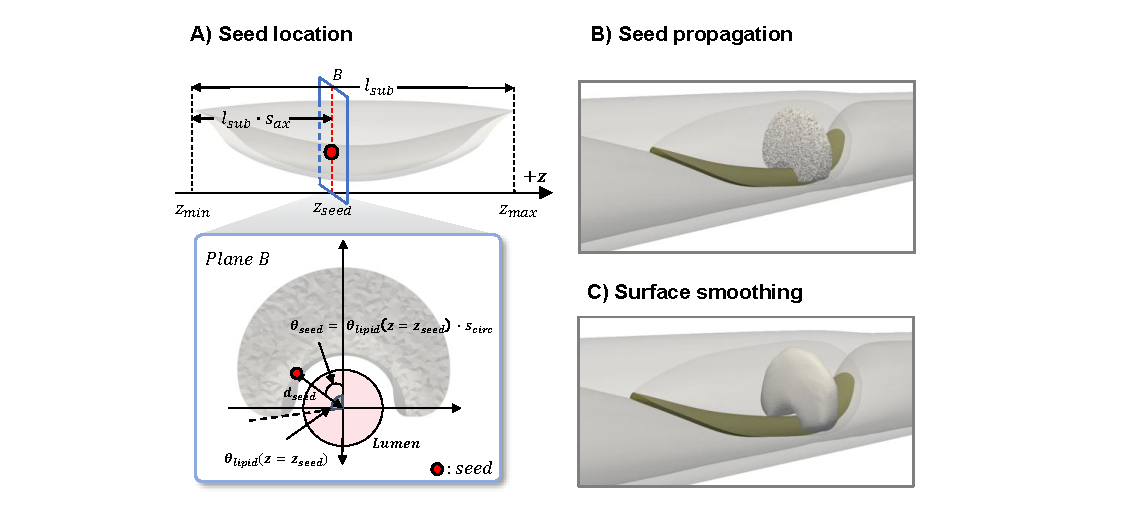
\includegraphics[width=\textwidth,height=0.82\textheight,keepaspectratio]{figures/figure_page_11.pdf}
\caption[Calcification generation algorithm]{Calcification generation: (A) seed location schematic, (B) seed propagation, (C) surface smoothing.}
\label{fig:appA-seed}
\end{figure}

\section{Generation procedure}
\begin{enumerate}
\item \textbf{Domain extraction (erosion).} Starting from the pre-generated lipid-core volume mesh (lesion region), the distance from each tetrahedral cell center to the fibrous-cap surface is computed with a KD-tree, and cells lying within $d_\mathrm{buf}$ of the fibrous-cap surface are removed. The remaining set of interior cells defines the region in which calcification may exist; this leaves a buffer so that the calcification does not touch the fibrous-cap/lipid boundary.
\item \textbf{Number of calcified cells.} $N_\mathrm{calc}=\operatorname{round}(f_\mathrm{calc}\times N_\mathrm{lipid,internal})$. The calcification volume is computed from the number of mesh cells that make up the calcification.
\item \textbf{(A) Seed placement.} The $z$ range of the interior region is normalized to $[0,1]$, and the axial position is set as $z_\mathrm{seed}=z_\mathrm{min}+(z_\mathrm{max}-z_\mathrm{min})\,s_\mathrm{ax}$. The circumferential angle is obtained by multiplying the lipid half-angle $\theta_\mathrm{lipid}(z_\mathrm{seed})$ of that $z$ cross-section by $s_\mathrm{circ}$, giving $\theta_\mathrm{seed}=s_\mathrm{circ}\,\theta_\mathrm{lipid}(z_\mathrm{seed})$; the distance from the lumen center to the seed at the $z=z_\mathrm{seed}$ cross-section is set as $d_\mathrm{seed}=r_\mathrm{lumen}(z_\mathrm{seed})+t_\mathrm{FC}+d_\mathrm{buf}$, yielding the seed coordinates $x_\mathrm{seed}=d_\mathrm{seed}\sin\theta_\mathrm{seed}$ and $y_\mathrm{seed}=d_\mathrm{seed}\cos\theta_\mathrm{seed}+y_c(z_\mathrm{seed})$. Here $t_\mathrm{FC}$ is the fibrous-cap thickness.
\item \textbf{(B) Anisotropic propagation.} A KD-tree is constructed in a transformed space in which the cell-center coordinates are scaled as $(x,y)\!\to\!\sqrt{w}\,(x,y)$, and the $N_\mathrm{calc}$ nearest cells to the transformed seed are selected. This grows the calcification blob according to a weighted distance criterion $\mathrm{dist}^2 \approx w(dx^2+dy^2)+dz^2$, allowing isotropic, axially dominant, and circumferentially dominant morphologies all to be produced. The selected cells are tagged as calcification.
\item \textbf{(C) Surface smoothing.} The set of calcified cells is extracted as a surface (STL) and the mesh surface is smoothed by Laplacian smoothing; the calcification volume is then measured for validation.
\end{enumerate}

\section{Calcification volume validation}

The generated calcification geometries were validated against prior imaging data. Because the calcified fraction $f_\mathrm{calc}$ was sampled uniformly over $[0.20, 0.80]$ of the lipid-core volume, the resulting absolute calcification volumes spanned a physiologically plausible range and followed a right-skewed distribution, with most lesions concentrated at smaller volumes and a long tail toward larger calcifications. Both this range and the right-skewed shape are consistent with the coronary artery calcium (CAC) volumes reported by Krishnamoorthy et al. (OCT-based, $n=250$ patients; CAC volume $\approx 0.01$--$0.0125\,\mathrm{cm}^3$), which exhibit the same right-skewed pattern within a comparable range. This agreement confirms that the synthetic calcification morphologies remained within clinically observed bounds~\cite{krishnamoorthy2017}.


\chapter{Inlet pressure and intramyocardial pressure generation}

Based on the hemodynamic parameters ($P_\mathrm{sys}$, $\Delta P$, and the decay ratio $\tau$), the corresponding inlet pressure $P_\mathrm{in}(t)$ and the myocardial pressure $P_\mathrm{myo}(t)$ for the lumped coronary boundary condition were generated. This appendix describes the specific algorithm used to derive them. The Windkessel, elastance, and coronary boundary-condition models themselves are standard and are cited in \S3.1.3; only the non-standard choices (fitting procedure and time rescaling) of this study are described here.

\section{Inlet pressure waveform: RCR fitting}
For a fixed coronary inflow waveform $Q(t)$, as shown in Fig.~\ref{fig:appB}(a), the three-element Windkessel is integrated with the following ODE~\cite{westerhof2009windkessel}:

\begin{equation}
\frac{dP_c}{dt} = -\frac{1}{\tau}\,(P_c - P_d) + \frac{Q(t)}{C}, \qquad P(t) = R_p\,Q(t) + P_c(t),
\end{equation}

where $\tau$ is the sampled diastolic time constant and $C=\tau/R_d$. The choices made in this study are as follows:
\begin{enumerate}
\item \textbf{Coronary ratio constraint:} $R_p/R_d = 1/10$ is fixed~\cite{westerhof2009windkessel}.
\item \textbf{Pressure-matching fit:} the decision variables $(P_d,\ \ln R_d)$ are determined by nonlinear least squares that minimize the normalized residual
\begin{equation}
r = \left[\frac{\max_t P - P_\mathrm{sys}}{|P_\mathrm{sys}|},\ \frac{\min_t P - P_\mathrm{dia}}{|P_\mathrm{dia}|}\right],
\end{equation}
so that the maximum and minimum of the periodically converged last-cycle pressure match the targets $(P_\mathrm{sys},\ P_\mathrm{dia})$, where $P_\mathrm{dia}=P_\mathrm{sys}-\Delta P$.
\item \textbf{Cycle convergence:} the single-beat $Q(t)$ is repeated for $n$ cycles (max $=50$) and integrated by forward Euler, with the terminal $P_c$ of the previous cycle carried over as the initial value of the next cycle, and the last cycle of the periodic steady state is taken.
\item \textbf{Time scaling and units:} the time axis is scaled by $T=60/\mathrm{HR}$, and the pressure is converted from mmHg to dyn/cm$^2$ ($\times1333.22$) and stored as solver input.
\end{enumerate}
As a result, $P_\mathrm{in}(t)$ is uniquely determined by the three variables $(P_\mathrm{sys},\ \Delta P,\ \tau)$.

\begin{figure}[!htbp]
\centering
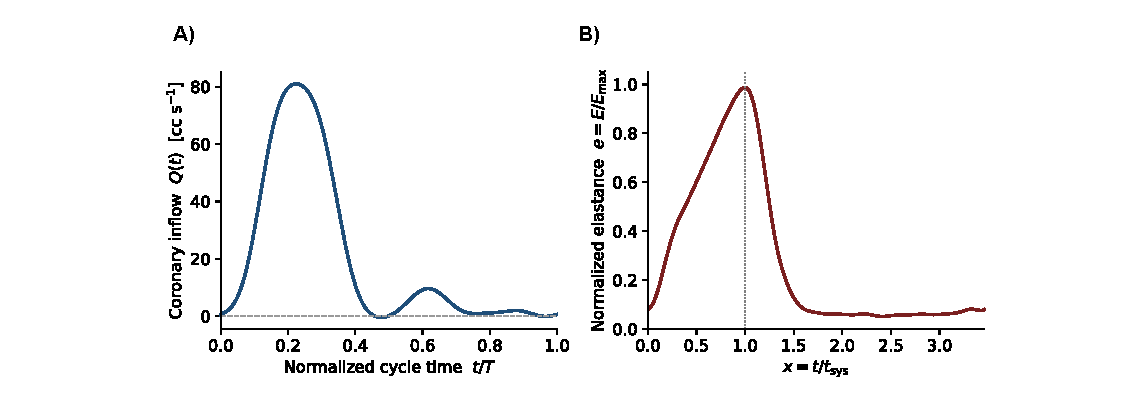
\includegraphics[width=\textwidth,height=0.82\textheight,keepaspectratio]{figures/figure_page_12.pdf}
\caption[Empirical inputs for pressure generation]{The two empirical inputs of Appendix B: (a) inflow waveform $Q(t)$; (b) normalized elastance $e(x)=E/E_\mathrm{max}$ ($x=t/t_\mathrm{sys}$; $x=1$ is end-systole).}
\label{fig:appB}
\end{figure}

\section{Myocardial pressure waveform}
Given the inlet pressure waveform $P_\mathrm{in}(t)$ generated in Appendix~B.1, the myocardial pressure waveform $P_\mathrm{myo}(t)$ was obtained by time-marching the lumped heart model used in the coronary boundary condition. The aortic pressure input of the heart model was prescribed as $P_\mathrm{ao}(t)=P_\mathrm{in}(t)$, and the ventricular pressure computed from the time-varying elastance model was used as the myocardial pressure, $P_\mathrm{myo}(t)=P_\mathrm{LV}(t)$. The governing heart-circuit equations followed the coronary lumped-parameter model of Kim et al.~\cite{kim2010coronary}; the corresponding model parameters are listed in Table~\ref{tab:appB-heart}, and the normalized elastance curve used in the heart model is shown in Fig.~\ref{fig:appB}(b). The heart-model state variables were then advanced in time using an explicit Euler-based time-marching scheme, with valve states updated at each time step. After repeated cycles reached a periodic steady state, the ventricular pressure from the last cycle was extracted as $P_\mathrm{myo}(t)$ for the coronary outlet boundary condition.

\begin{table}[ht]
\caption[Lumped heart model constants]{Lumped heart model constants~\cite{kim2010coronary}.}
\label{tab:appB-heart}
\begin{center}
\begin{tabular}{lllrl}
\hline\hline
Category & Parameter & Symbol & Value & Unit \\
\hline
Ventricle & Maximum elastance & $E_\mathrm{max}$ & 2.0 & mmHg/mL \\
Ventricle & Systolic duration & $t_\mathrm{sys}$ & 0.4 & s \\
Ventricle & Resistance & $R_v$ & 40.0 & CGS \\
Ventricle & Inertance & $L_v$ & 0.01 & CGS \\
Atrium & Elastance & $E_a$ & 250 & CGS \\
Atrium & Resistance & $R_a$ & 5.0 & CGS \\
Atrium & Inertance & $L_a$ & 0.1 & CGS \\
Global & Heart rate & HR & 60 & bpm \\
Global & Cardiac output & CO & 5 & L/min \\
Initial condition & Ventricular/atrial volume & $V_v(0)/V_a(0)$ & $0\,/\,{-}60$ & mL \\
\hline\hline
\end{tabular}
\end{center}
\end{table}


%%======================================================================
%% Bibliography — author will supply references.bib
%%======================================================================
%% NOTE: All in-text citations are left as \cite{...}. Replace the block
%% below with \bibliographystyle{...} and \bibliography{references} once
%% the .bib file is added.
%%
\bibliographystyle{unsrt}
\bibliography{references}


%%======================================================================
%% 감사의 글
%%======================================================================
\acknowledgment[1]
먼저 부족한 저를 받아 주시고 연구의 길을 이끌어 주신 김현진 교수님께 진심으로 감사의 말씀을 드립니다. 연구의 방향을 잡지 못하고 헤맬 때마다 따뜻한 조언과 날카로운 가르침으로 길을 밝혀 주신 덕분에 이 학위논문을 마칠 수 있었습니다. 교수님께 배운 학문에 대한 태도와 자세를 앞으로의 삶에서도 잊지 않고 간직하겠습니다.

또한 바쁘신 와중에도 본 논문을 심사해 주시고 소중한 의견을 주신 심사위원 교수님들께 깊이 감사드립니다. 함께 연구하며 즐거움과 어려움을 나눈 CBML 연구실 동료들에게도 고마운 마음을 전합니다.

끝으로, 언제나 변함없는 사랑과 믿음으로 저를 지지해 주신 부모님과 가족들에게 가장 큰 감사를 드립니다. 묵묵히 응원해 주신 가족이 있었기에 오늘의 제가 있을 수 있었습니다. 이 작은 결실을 사랑하는 가족과 함께 나누고 싶습니다.

\hfill 2026년 6월\\
\hfill 김 세 혁 올림


%%======================================================================
%% 약력
%%======================================================================
\curriculumvitae[1]

\begin{personaldata}
    \name       {김 세 혁}
    \dateofbirth{1999}{12}{28}
    \birthplace {대한민국}
    \address    {(34141) 대전광역시 유성구 대학로 291, 한국과학기술원 갈릴레이관(W3)}
\end{personaldata}

\begin{education}
    \item[2018. 3.\ --\ 2024. 8.] 성균관대학교 기계공학과 (학사)
    \item[2024. 8.\ --\ 2026. 8.] 한국과학기술원 기계공학과 (석사)
\end{education}

\label{paperlastpagelabel}
\end{document}
